\documentclass[twoside, final, 11pt]{articleMine}
\usepackage[english]{babel} \usepackage{a4wide}
\usepackage{amsmath,amssymb,accents} \usepackage{epsfig}
\usepackage{subfigure} \usepackage{units} \usepackage{graphicx}
\usepackage[displaymath, mathlines, right]{lineno} \usepackage{xspace}
\usepackage{color} \usepackage{epic,eepic,pstricks}
\usepackage{acronym} \usepackage{wrapfig,multicol}
\usepackage{deluxetable} \usepackage{todonotes} 
\usepackage{hyperref}
%\usepackage{slashbox}
\usepackage{lmodern} 
%\usepackage{caption}
\linenumbers
%\usepackage{showlabels}
\usepackage[draft]{showkeys}

%\usepackage[nolists, tablesfirst]{endfloat}
\graphicspath{{plots/}}
\newcommand*\patchAmsMathEnvironmentForLineno[1]{%
  \expandafter\let\csname old#1\expandafter\endcsname\csname #1\endcsname
  \expandafter\let\csname oldend#1\expandafter\endcsname\csname end#1\endcsname
  \renewenvironment{#1}%
     {\linenomath\csname old#1\endcsname}%
     {\csname oldend#1\endcsname\endlinenomath}}%
\newcommand*\patchBothAmsMathEnvironmentsForLineno[1]{%
  \patchAmsMathEnvironmentForLineno{#1}%
  \patchAmsMathEnvironmentForLineno{#1*}}%
\AtBeginDocument{%
\patchBothAmsMathEnvironmentsForLineno{equation}%
\patchBothAmsMathEnvironmentsForLineno{align}%
\patchBothAmsMathEnvironmentsForLineno{flalign}%
\patchBothAmsMathEnvironmentsForLineno{alignat}%
\patchBothAmsMathEnvironmentsForLineno{gather}%
\patchBothAmsMathEnvironmentsForLineno{multline}%
}
%\AtBeginFigures{\cleardoublepage}
%%%%%\parindent 5pt  
\parskip 1.2pt           % sets spacing between paragraphs
\def\Offline{\mbox{$\overline{\rm
Off}$\hspace{.05em}\raisebox{.4ex}{$\underline{\rm line}$}}\xspace}
\def\OfflineB{\mbox{$\bf\overline{\rm\bf
Off}$\hspace{.05em}\raisebox{.4ex}{$\bf\underline{\rm\bf line}$}}\xspace}

\def\eq#1{\begin{equation}#1\end{equation}}
%\def\al#1{\begin{align}#1\end{align}}
%\def\vc#1{{\bf #1}}
\def\pt#1{\accentset{\rightharpoonup}{#1}}
\include{myabbr}

\newcommand{\HRule}{\rule{\linewidth}{0.5mm}}
\newcommand{\VEM}{\mbox{VEM}}
\newcommand{\m}{\mbox{m}}

\let\stdsection\section  
%\renewcommand\section{\newpage\stdsection}  
 
\begin{document}

%\setpagewiselinenumbers
\modulolinenumbers[2]

%\linenumbers


\renewcommand\linenumberfont{\small\rmfamily}
\begin{center}
  \vspace*{-13ex}

  \rule{\linewidth}{0.1mm}  \\[17mm] {\huge  Detector simulation and validation with dat}
     \begin{flushright}
       \small 
     
     \end{flushright}

  % 
\end{center}
% 
\vspace*{2ex} 
%
\thispagestyle{empty}
\noindent
\begin{abstract}
  \noindent
We detail  in this note the  simulation method of  the EASIER detector
from the Radio Frequency (RF) signal to the ADC trace. We validate and
compare  our  models with  the  data  of  the three  different  C-band
detectors.
\end{abstract}

%
\thispagestyle{empty}
%$\;$
%\listoftodos
%\newpage
\noindent
\section{Introduction}
The  current  signal  search for  EASIER  event  is  based on  a  peak
detection. To be  considered as an event, a peak  also needs to arrive
in coincidence with the trigger given by the particle signal and above
a fixed threshold.  It is robust  but it is not the best technique for
the search of small signals.  We study in this note the improvement of
the signal  to noise  ratio when  a matched filter  is applied  to the
radio trace.  %% This method can be applied to all type of EASIER
%% detectors  (EASIER/GD  C-band/GD helix).
\\ In  the first section  we present briefly the  detector simulations
needed  to   test  the   effect  of  the   filters.   Then   we  study
quantitatively    the   improvement    in   sensitivity    with   mock
signals. Finally, we apply these methods to realistic simulation data.

\section{RF simulation}
\label{sec:rf}
We detail here the way to  simulate the RF noise signal, we will first
show  the ideal  case  of a  flat  spectrum and  find numerically  the
formula of the ratio of the rms over the mean. Then we will see how to
simulate a realistic spectrum.
\subsection{Theory}
\label{sec:theory}
One way to  check our simulation is by looking at  what is expected in
term of  signal distribution.  In  simple cases of input  spectrum and
detector,  the  RMS  and the  mean  of  the  waveform can  be  derived
analytically.\\  A derivation  is given  in the  book "Tools  of Radio
Astronomy" (T.L~Wilson, K.~Rohlfs,  S.~Huttemeister).  As we will see,
a convenient value to  look at is the ratio of the  RMS over the mean,
because some calibration parameters  like the temperature and the gain
will cancel  out.  Finally knowing  the RMS of  your signal is  a good
estimation of your  sensitivity. The main steps of  the derivation are
the following:
\begin{itemize}
\item take a  radio detector with a bandwidth B,  the amplitude of the
  signal $v(t)$ follows a gaussian distribution.
\item the signal goes through a square law detector $y = av(t)^2$. One
  can  compute the  mean  and  standard deviation  and  finds: $<y>  =
  a\sigma_v^2$ and $\sigma_y = \sqrt{2}a\sigma_v^2$ (with $<v^2> = <power> =
  kT_{sys}     G    B$).    (this     webpage    might     also    help:\\
  \url{http://mathworld.wolfram.com/GaussianIntegral.html})
\item So we have: $\sigma_y = \sqrt{2} <y> $ , with $\sigma_y = k_B \Delta
  T G B$ so $\Delta T = \sqrt{2} T_{sys}$
\item now  if we  average over  a time $\tau$,  that means  we average
  over$ N = f_{Nyquist}*\tau$ points where $f_{Nyquist} = 2B$, and we reduce the fluctuation by a factor $\sqrt{N}$
\item we finally obtain: $\Delta T = \frac{T_{sys}}{\sqrt{B\tau}}$
\end{itemize}
To  sum up,  for a  input  gaussian signal  followed by  a square  law
detector we expect the  ratio $\rm \frac{\sigma}{\mu} = \sqrt{2}$. And
this  ratio  is then  modified  by  the  later processing,  averaging,
filtering. The formula that is commonly used is:
\begin{equation}
  \frac{\sigma}{\mu} = \frac{1}{\sqrt{\Delta B \cdot \tau}}
  \label{eq:sigmamu}
\end{equation}
We verify in the next paragraph the validity of this expression.

\subsection{flat spectrum}
\paragraph{no filter}
We start with the case of a flat spectrum with a phase drawn randomly.
We  produce a  waveform  from  the spectrum  by  inverse Fast  Fourier
Transform.  An example of such a waveform and its spectrum is shown in
the    figure.~\ref{fig:flatspec}.    One    can   check    that   the
$\frac{\sigma}{\mu}$  ratio is  $\sqrt{2}$ as  expected.  We  can also
check that this ratio doesn't  depend on the chosen bandwidth as shown
in fig.~\ref{fig:bwfilt} left.
\begin{figure}[!ht]
  \centering
  \hspace*{-3ex}
  \subfigure{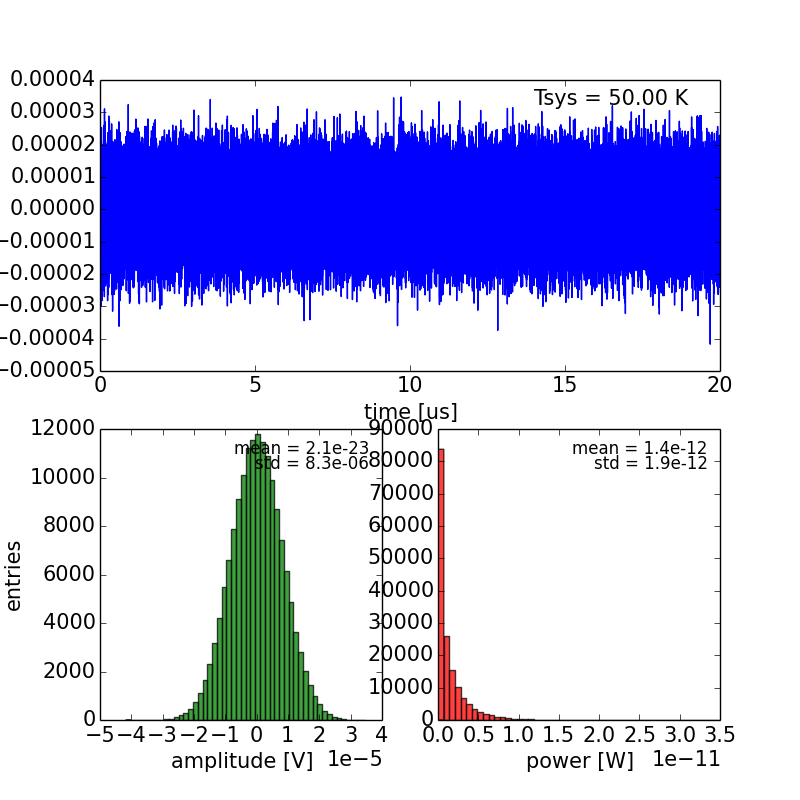
\includegraphics[width=0.49\linewidth]{noise.png}}
  \subfigure{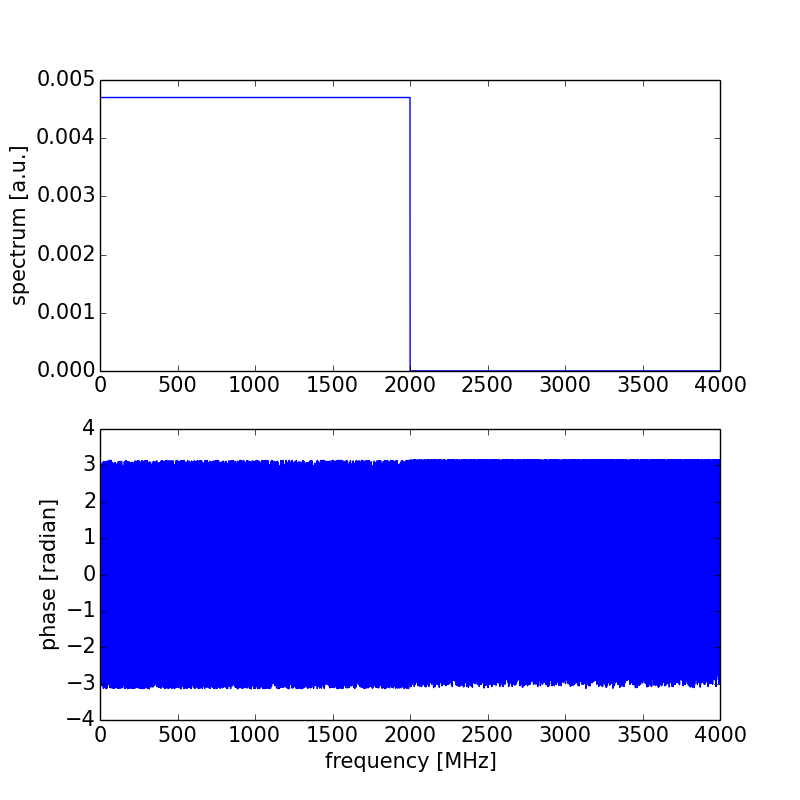
\includegraphics[width=0.49\linewidth]{specphasenoise.png}}
  \caption{Left: top:  waveform, bottom left:  amplitude distribution,
    bottom  right power  distribution. Right:  top:  spectrum, bottom:
    phase}
  \label{fig:flatspec}
\end{figure}


\begin{figure}[!ht]
  \centering
  \hspace*{-3ex}
  \subfigure{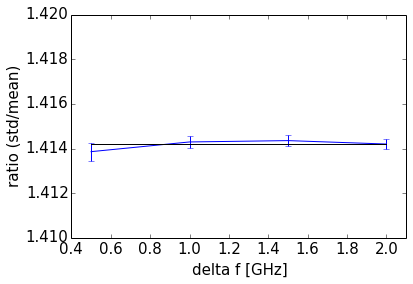
\includegraphics[width=0.49\linewidth]{ratiodiffBW.png}}
  \subfigure{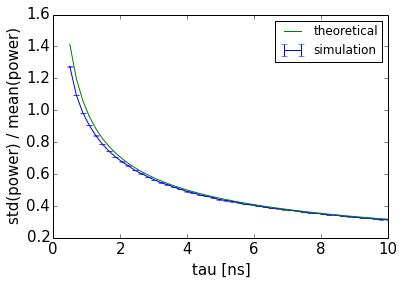
\includegraphics[width=0.49\linewidth]{rationumfilter.png}}
  \caption{left: ratio $\frac{\sigma}{\mu}$ versus the lower frequency
    $f_min$ of the noise spectrum. rigt: the ratio when we apply a low
    pass filter of frequency cut $f_{cut}= 1/\tau$ to the power. It is
    shown for three different $f_{min}$}
  \label{fig:bwfilt}
\end{figure}

\paragraph{numerical filter}
Now we  filter the  waveform (  after converting it  to power)  with a
numerical filter  (we set  the fft coefficient  to 0 for  the filtered
frequencies.).  The orignal waveform is issued from a spectrum between
0    and   2GHz.    We    show   in    fig.~\ref{fig:bwfilt}   (right)
$\frac{\sigma}{\mu}$  the ratio  for different  frequency cuts  of the
filter  where   the  x-axis  is  the   time  constant  $   \rm  tau  =
\frac{1}{f_{cut}}$.   We see that  it follows  very well  the expected
formula.\\ Now if  we vary the bandwidth and then  apply the filter we
obtain the result in the  fig.~\ref{fig:bwfilt2} (left).  We see now a
discrepancy between the expected ratio  and the simulated one.  We see
that if we reduce the bandwidth,  the ratio is lower than expected and
plateaus at  for the high  frequency filters (low $\tau$)  but matches
the formulas at  the low frequency filter (high  $\tau$).  This can be
understood  when  we  think  about  the  FFTs  (or  look  at  them  on
figure~\ref{fig:bwfilt2}).  The  fourier transform of the  power for a
signal at  frequencies in [f1  - f2] has  a contribution between  [0 ;
  $\Delta  B/2$], where  $\Delta B  = f2-f1$  and another  one between
[2*f1 ; 2*f2].  On the figure we see an example for an amplitude input
spectrum of  [1.5 ; 2  GHz].  If we  filter the power spectrum  with a
frequency  $f_{cut} $smaller  than  $\Delta B/2$  then  we follow  the
equation because  we have a full  or a continuous bandwidth  from [0 ;
  $f_{cut}$], if $f_{cut}$  is larger then we go into  the hole in the
power spectrum and  we don't add any frequency  in the average, that's
why the ratio goes to a constant.

\begin{figure}[!ht]
  \centering
  \hspace*{-3ex}
  \subfigure{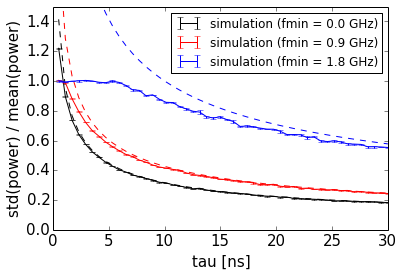
\includegraphics[width=0.49\linewidth]{rationumfilterdiffBW.png}}
  \subfigure{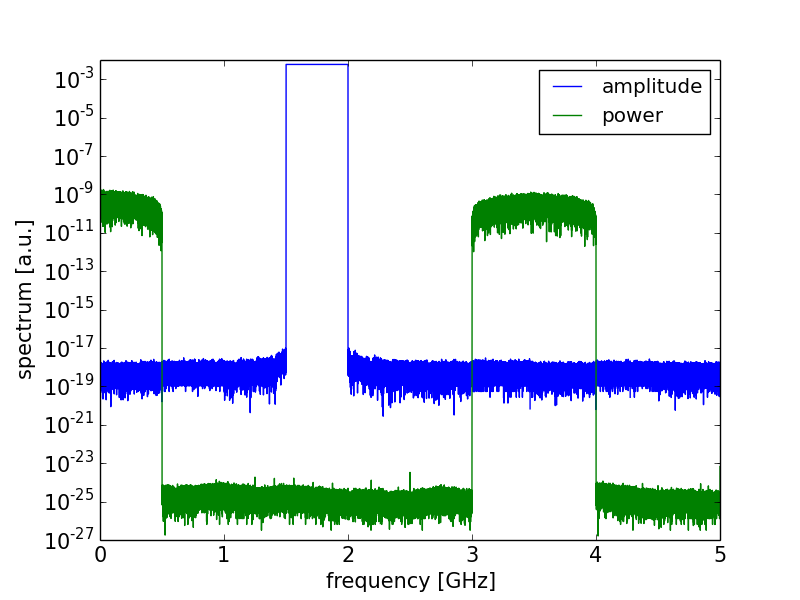
\includegraphics[width=0.49\linewidth]{specnoise.png}}
  \caption{left: ratio $\frac{\sigma}{\mu}$ versus the lower frequency
    $f_min$ of the noise spectrum. rigt: the ratio when we apply a low
    pass filter of frequency cut $f_{cut}= 1/\tau$ to the power. It is
    shown for three different $f_{min}$}
  \label{fig:bwfilt2}
\end{figure}

\paragraph{sliding window}
In  this paragraph,  instead  of filtering  by  cutting the  frequency
spectrum  we average over  several time  bins, i.e.  we use  a sliding
window  average.  If  we consider  $\tau$ as  the window  size  we see
(fig~\ref{fig:slidingwindow})  that  the   ratio  doesn't  follow  the
equation~\ref{eq:sigmamu}.  There is an additional factor to be added.
\begin{figure}[!ht]
  \centering
  \hspace*{-3ex}
  \subfigure{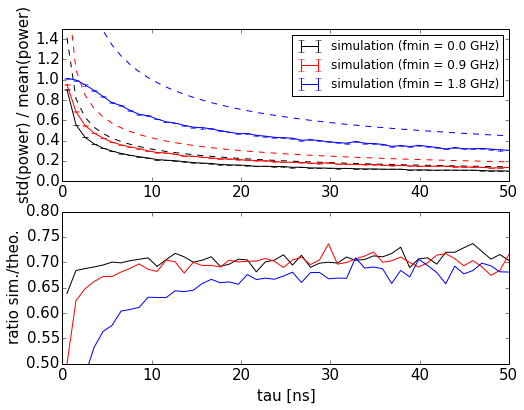
\includegraphics[width=0.60\linewidth]{slidingwindow.png}}
  \caption{$\frac{\sigma}{\mu}$ ratio after  applying a sliding window
    of size $\tau$ for different $f_{min}$}
  \label{fig:slidingwindow}
\end{figure}

We showed that the formula~\ref{eq:sigmamu}  can not be always used in
this  form. Some  conditions have  to  be matched  and the  processing
technique  (filtering  or other  sort  of  averaging)  can change  the
ratio.\\ It  can still  be used  as a figure  of merit  but it  is not
anymore representative  of the minimum  detectable signal (or  the one
sigma deviation from the mean).

\subsection{realistic spectrum}
Our detectors  have not  a flat spectrum  (cf fig.~\ref{fig:spectra}).
We first show  how we simulate it  and then we see how  to account for
this in the equation~\ref{eq:sigmamu}.

\paragraph{detectors gain}
The spectrum  that we need to  simulate our signal is  the spectrum at
the  input of  the power  detector. We  show here  that  this spectrum
depends only  on the antenna  and LNB gain.  \\ What comes out  of the
antenna + LNB is:
\begin{equation}
   \rm P(\nu) = \frac{1}{2}\int_\Omega F(\nu) A_{eff}(\nu) G_{LNB}(\nu)d\Omega
\end{equation}
with
\begin{equation}
  \rm F(\nu) = \frac{2k_B T \nu^2}{c^2}
\end{equation}
and

\begin{equation}
  \rm A_{eff}(\nu) = \frac{ G_{ant}(\nu)c^2 }{4\pi \nu^2 }
\end{equation}


So the  $\rm \nu^2$ cancels  out and we  have only:
\begin{equation}
   \rm P(\nu) = \frac{1}{4\pi}\int_\Omega k_B T G_{ant}(\nu) G_{LNB}(\nu) d\Omega= k_B T_{ant} G_{LNB}(\nu)
\end{equation}
Then the only dependence in frequency is given by the antenna gain and
the  amplifier gain.   For  the three  antenna  and LNB  that we  have
installed we have this data with:
\begin{itemize}
\item for EASIER antennas (DMX and GI301):spectrum measurement (in the field or at room temperature)
\item for GIGADuck antenna (Norsat) : IMEP measurement of the total gain antenna+LNB
\end{itemize}

\begin{figure}[!ht]
  \centering
  \hspace*{-3ex}
  \subfigure{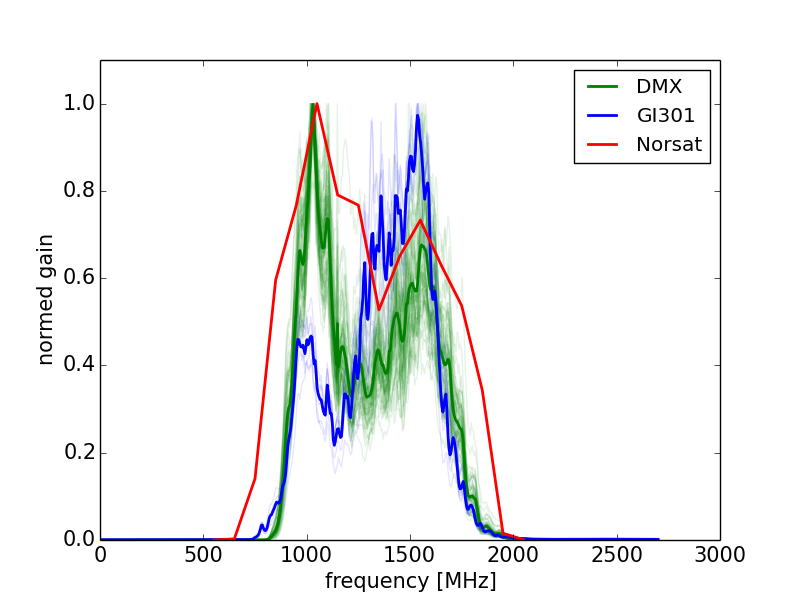
\includegraphics[width=0.60\linewidth]{spectra3.png}}
  \caption{gain spectra for the three types of LNB in the C-band.}
  \label{fig:spectra}
\end{figure}

\paragraph{simulation with realistic spectrum}
To simulate  a waveform with the  detector spectrum, we  set first the
fft with the  \textbf{square root of the power gain}  and the phase is
again drawn randomly from a uniform distribution between [$ \rm -\pi ;
  \pi$].
\paragraph{what is the bandwidth ?}
Now  we want  to know  how  to relate  the realistic  bandwith to  the
equation~\ref{eq:sigmamu}.  Usually  we take  the bandwith as  800 MHz
because of the definition of  the C-band (3.4-4.2 GHz). However we see
that the gain is not flat so what quantity should we take to enter the
equation~\ref{eq:sigmamu}  ?   One  can  think   about  the  following
definition:
\begin{equation}                                                                           
  \rm \Delta B = \frac{1}{G_{max}} \int G(\nu) \cdot d\nu  
  \label{eq:eqdeltab} 
\end{equation} 
This definition is usefull for instance to estimate the total power in
a band. For instance this  bandwidth will enter the calculation of the
average    power    (see    second    point    of    the    derivation
section\ref{sec:theory}) \\In  fact we  need to compute  the bandwidth
as:
\begin{equation}
  \rm \Delta B = \frac{1}{\sqrt{G_{max}}} \int \sqrt{G(\nu)} \cdot d\nu
  \label{eq:eqdeltabsqrt}
\end{equation}
To see this we can look  at the $\frac{\sigma}{\mu}$ ratio from a real
waveform of noise  coming from an antenna (a  DMX antenna) and compare
it with  the $\frac{\sigma}{\mu}$ ratio  of a flat  spectrum generated
waveform   with  $\Delta  B$   computed  as   eq~\ref{eq:eqdeltab}  or
eq~\ref{eq:eqdeltabsqrt}. (We need to apply a filter so that the ratio
is different from $\sqrt{2}$).
\begin{figure}[!ht]
  \centering
  \hspace*{-3ex}
  \subfigure{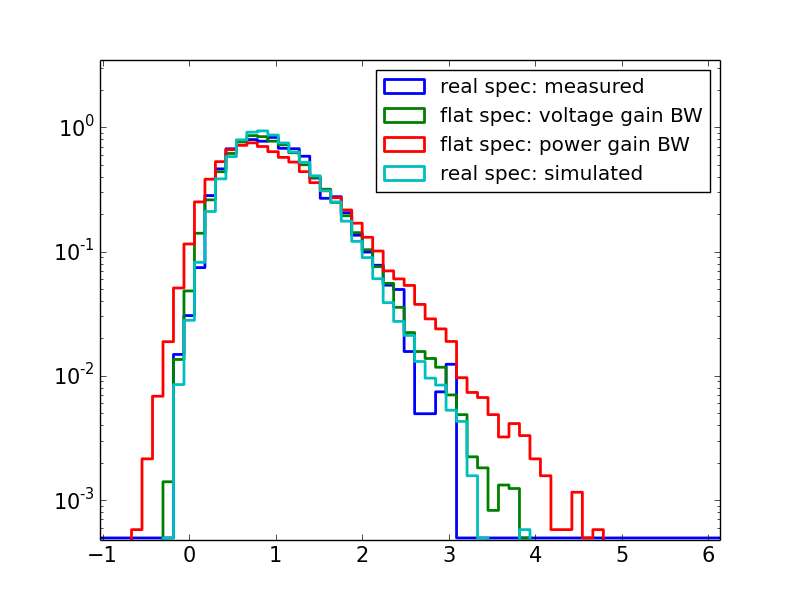
\includegraphics[width=0.60\linewidth]{noisedist.png}}
  \caption{noise distribution after power  filtering in 4 cases: blue:
    real waveform  from a DMX antenna. green:  flat spectrum generated
    waveform with bandwidth according eq~\ref{eq:eqdeltabsqrt}, red:flat
    spectrum    generated    waveform    with   bandwidth    according
    eq~\ref{eq:eqdeltab},  light  blue:   waveform  generated  from  the
    spectrum in fig~\ref{fig:spectra}}
  \label{fig:spectra}
\end{figure}
At the end the bandwidth are given is the table~\ref{tab:tabdeltab}.
\begin{table}[h!]
  \centering
  \caption{bandwidths}
  \label{tab:tabdeltab}
  \begin{tabular}{|c||c|c|c|}
    \hline
    antenna type & GI301  & DMX & Norsat \\
    \hline
    voltage bandwidth & 704 $\rm \pm 29$& 689 $\rm \pm$ 46 & 901\\
    \hline
    power bandwidth & 437 $\rm \pm 30$& 445 $\rm \pm$ 56 & 684\\
    \hline
  \end{tabular}
\end{table}








\section{Adaptation electronics simulation}
\label{sec:elec}
Here we  consider the adaptation  electronics starting from  the power
detection up  to the analog to  digital conversion and  the final data
see fig.~\ref{fig:detscheme}.  In this chain, the main components are:
the power detector, the adaptation  board, the SD front end filter and
the ADC.   Some other  minor elements (minor  in the sense  they won't
modify the  signal shape or SNR  but only its  amplitude, like cables,
75-50 adapter or other lossy element) won't be simulated.
\subsection{power detection}
The step of the power detection is the most specific to EASIER system.
We present  here three methods  to simulate the power  detector.  They
are  closely related,  two of  them are  based on  a convolution  in a
simular way  I had done in  my thesis. The  third one is based  on the
frequency response.  To  test the methods we have  calibration data we
had taken  back in 2013.  The setup is  composed of a  C-band antennna
followed by a  power detector.  The signal is  recorded with the large
bandwidth oscilloscope simultaneously after  the antenna and the after
the  power   detector.   We  have  data  with   only  backgroud  noise
(fig.~\ref{fig:signalexample} left) and data with short pulses emitted
with an electronic lighter (fig.~\ref{fig:signalexample} right).
\begin{figure}[!ht]
  \centering
  \hspace*{-3ex}
  \subfigure{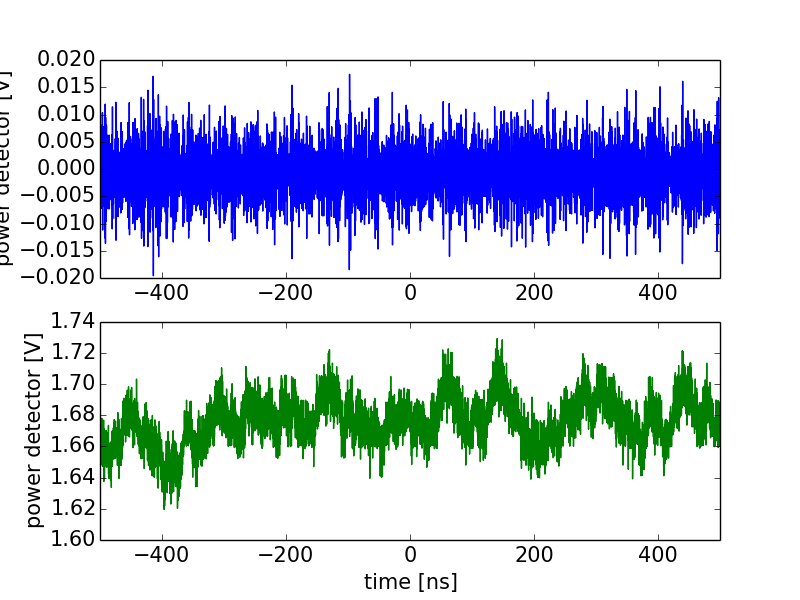
\includegraphics[width=0.49\linewidth]{noiseRFPD.png}}
  \subfigure{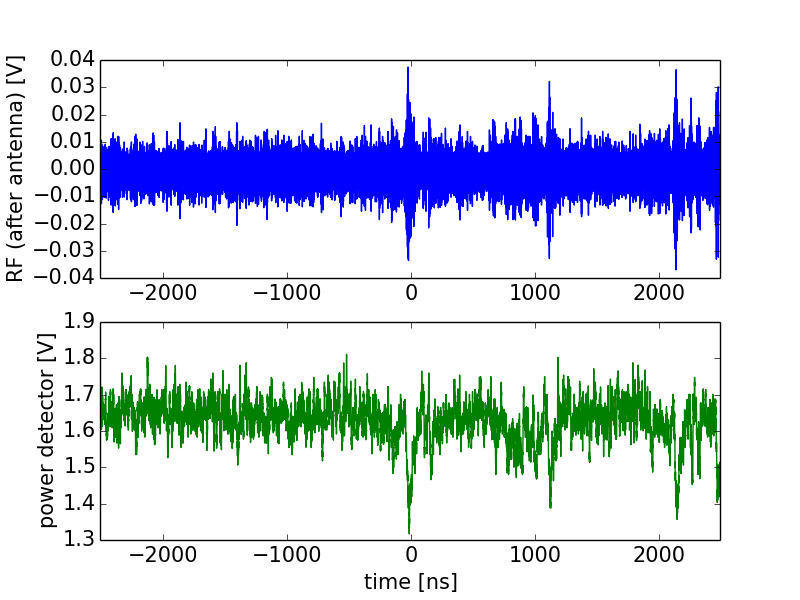
\includegraphics[width=0.49\linewidth]{signalexample.png}}
  \caption{example of calibration data, with only background noise (left), and with pulses (right)}
  \label{fig:signalexample}
\end{figure}

\subsubsection{DC calibration}
We first look at the calibration  of the DC component. We will use the
noise data to determine it. The method is very simple we just plot the
average  of the  power detector  waveform  against the  RF average  in
dBm. The  only interesting detail  here is the difference  between the
average of the log ($\rm <P> = \frac{1}{N}\Sigma P_{dBm}$) and the log
of the  average ($\rm <P>  = \frac{10}{N} \log_10 \Sigma  P_{mW}$). We
see these  characteristics on the  figure~\ref{fig:pdcarac}.  The main
difference  is   the  offset,  the   slope  found  from  the   fit  is
approximately the same.
\begin{figure}[!ht]
  \centering
  \hspace*{-3ex}
  \subfigure{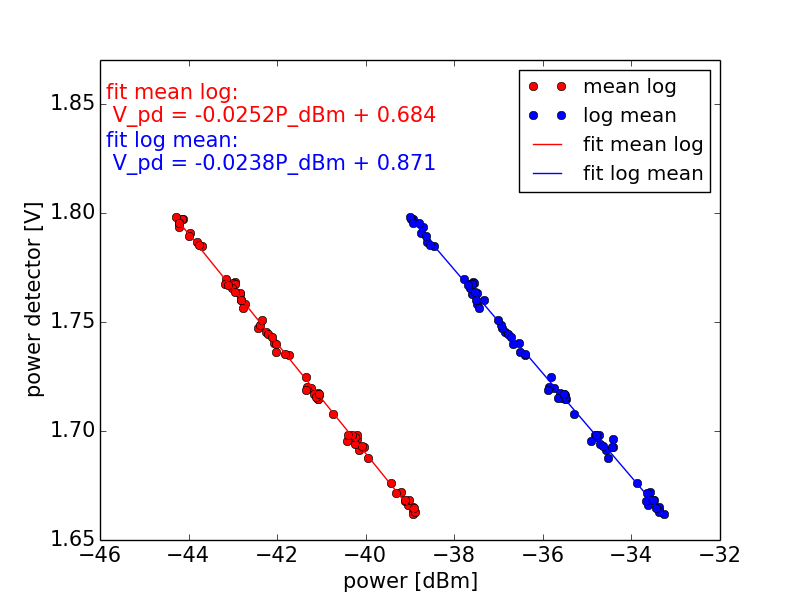
\includegraphics[width=0.60\linewidth]{powerdetDCcarac.png}}
  \caption{caracteristics of the power detector in the case we take the log of the mean power or in the case we take the mean of the log power}
  \label{fig:pdcarac}
\end{figure}
This  characteristics is  only  valid to  relate  the baseline  value,
i.e. mean values. If we want  to reproduce the waveform, we need a bit
more  complicated methods. We  present some  example in  the following
paragraphs.

\subsubsection{convolution with floating parameters (method 1)}
We  found  that a  good  way  to simulate  the  power  detector is  by
performing  a convolution  of the  signal in  dBm with  an exponential
decay function.   \\ We  want to reproduce  the power  detector signal
from the RF signal. Here are the steps we follow:
\begin{itemize}
\item transform RF signal in dBm
\item do the convolution with $f(t) = A\cdot \exp{\frac{t}{\tau}}$
\item  transform linearly  the  result to  obtain  the power  detector
  waveform: $V_{sim} = a\cdot V_{conv} + b$
\end{itemize}
In order to  find the parameters $\tau$,  a and b, we scan  a range of
values of  $\tau$, and then  fit $V_{conv}$ versus $V_{PD}$.   Then we
search for $\tau$, a and b  that minimize the distance $\rm d = \Sigma
(V_{sim} -  V_{PD})^2$ between the  two waveforms.  This  procedure is
perfomed on  20 waveforms  and the average  parameters are  chosen (cf
table~\ref{tab:method1tab}).
\begin{table}[h!]
  \centering
  \caption{parameters for the power detection}
  \label{tab:method1tab}
  \begin{tabular}{|c||c|c|c|}
    \hline
    & $\tau$ [ns] & a & b \\
    \hline
    with capacitor & $\rm 4.7 \pm 0.2$ & $\rm -0.019 \pm 0.001 $ & $\rm 0.88 \pm 0.04 $ \\
    \hline
    without capacitor & $\rm 35.2 \pm 2.2$ & $\rm -0.022 \pm 0.001 $  & $\rm 0.79 \pm 0.04 $\\
    \hline
  \end{tabular}
\end{table}
An example of a resulting simulated signal overlayed with the original
one is shown in the fig.~\ref{fig:m1ex} (middle) and the difference is
shown in the fig.~\ref{fig:m1ex} (bottom).
\begin{figure}[!ht]
  \centering
  \hspace*{-3ex}
  \subfigure{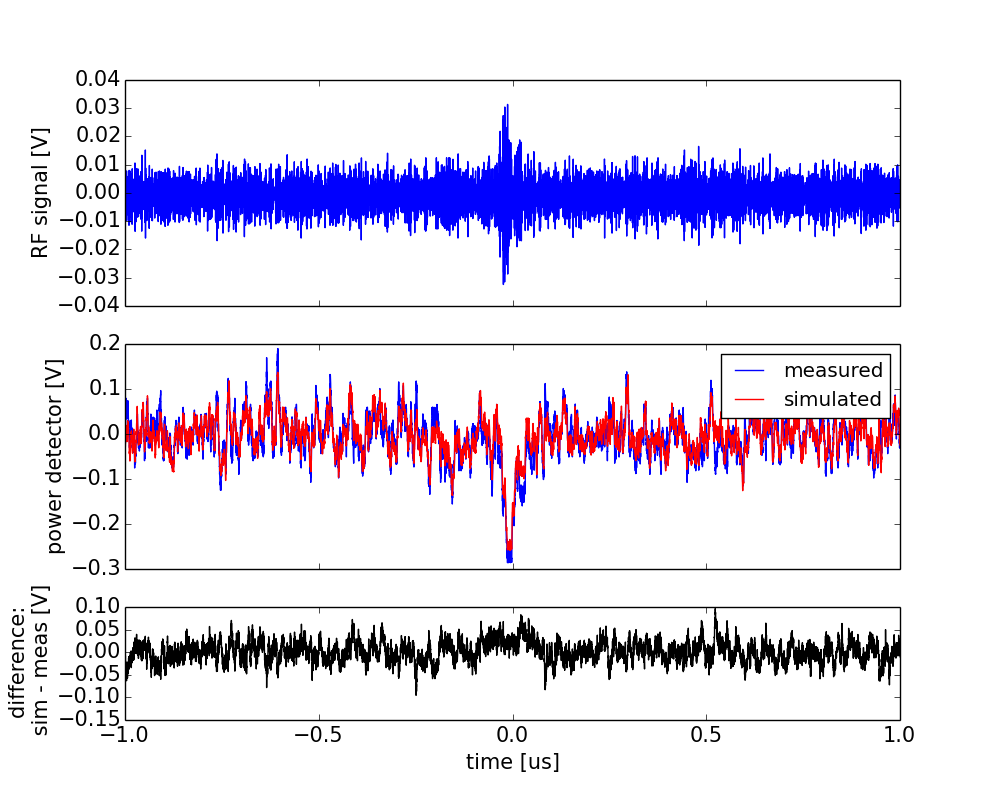
\includegraphics[width=0.49\linewidth]{nocapa_method1.png}}
  \subfigure{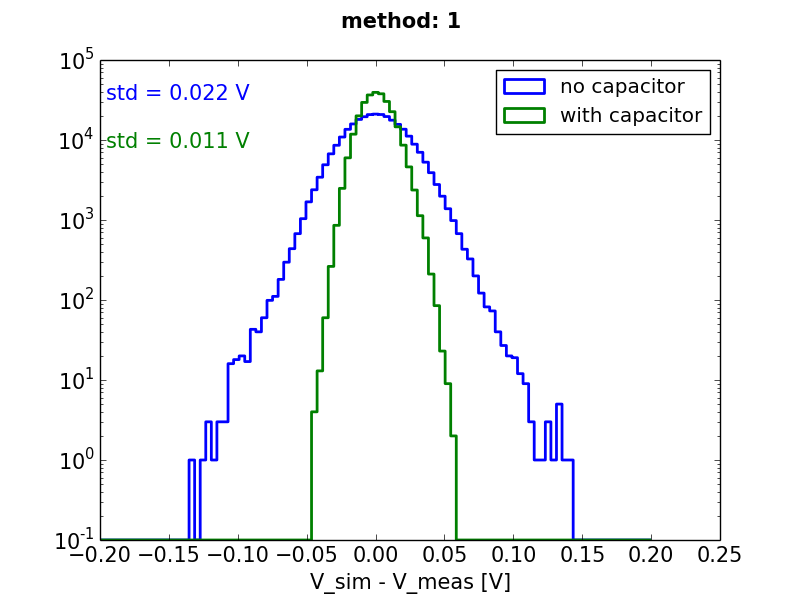
\includegraphics[width=0.49\linewidth]{res_method1.png}}
  \caption{top:  RF  waveform,  middle:  power detector  measured  and
    simulated, bottom: difference}
  \label{fig:m1ex}
\end{figure}
When  using the  average parameters  to all  waveforms, we  obtain the
residuals distribution in the figure~\ref{fig:m1ex}. The standard
deviation  for  the  no  capacitor  case  is 22mV  and  11mV  for  the
capacitor.

\newpage
\subsubsection{transfer function method}
Another way  to simulate  the power detector  response can be  done by
looking at the transfer function  in the frequency domain. This can be
seen  as a  filter  response.  In  practice,  we need  to  use the  DC
caracteristics we  already found (cf  fig.~\ref{fig:pdcarac}) and then
look  at the frequency  spectrum of  the signal  before and  after the
power detector.  Note that the  RF signal is first transformed in dBm,
i.e. in logarithmic  scale. We use the waveforms  presented before for
the convolution method.  On  the figures~\ref{fig:pdspec1} we show the
spectra  before  and  after  the  power  detector  (left),  the  ratio
(middle),     an      example     of     the      phase     difference
(right). Fig.~\ref{fig:pdspec1} is the  case when the capacitor is used
and fig.~\ref{fig:pdspec2} is  the no  capacitor  case. We  see that  the
capacitor case filters at lower frequencies as expected.
\begin{figure}[!ht]
  \centering
  \hspace*{-3ex}
  \subfigure{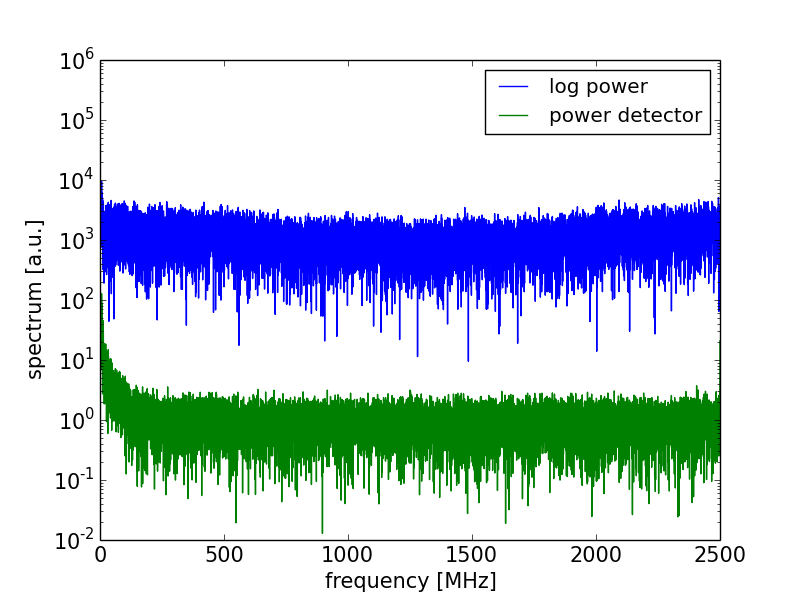
\includegraphics[width=0.32\linewidth]{c_spec.png}}
  \subfigure{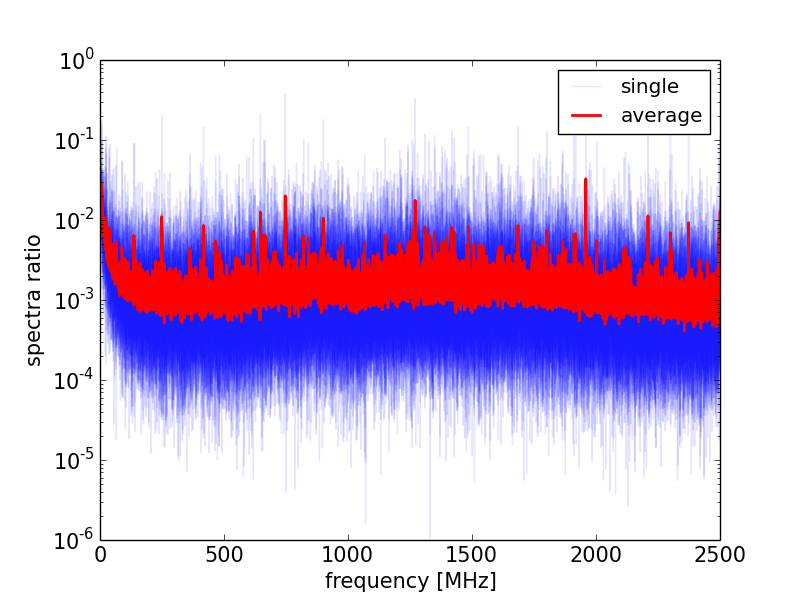
\includegraphics[width=0.32\linewidth]{c_ratio.png}}
  \subfigure{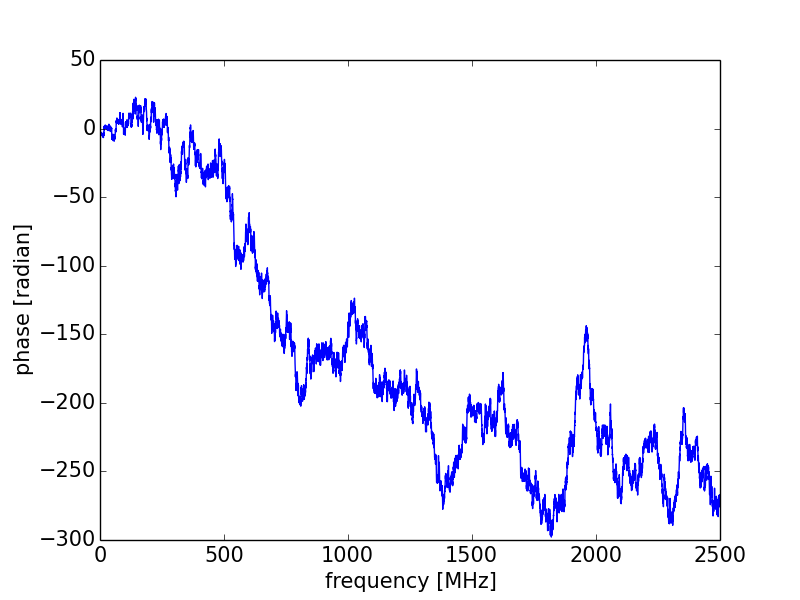
\includegraphics[width=0.32\linewidth]{c_phase.png}}
  \caption{capacitor case (left: spectrum, middle: ratio after/before, right: phase difference)}
  \label{fig:pdspec1}
\end{figure}

\begin{figure}[!ht]
  \centering
  \hspace*{-3ex}
  \subfigure{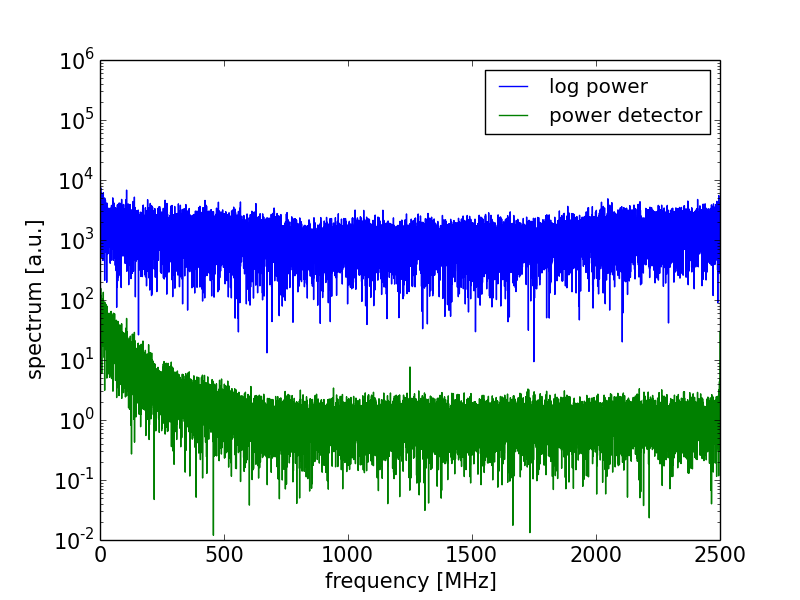
\includegraphics[width=0.32\linewidth]{nc_spec.png}}
  \subfigure{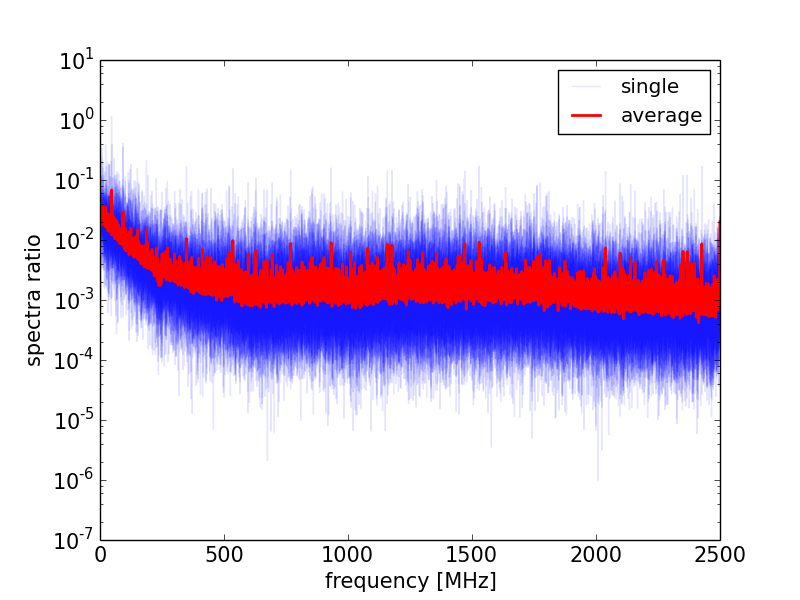
\includegraphics[width=0.32\linewidth]{nc_ratio.png}}
  \subfigure{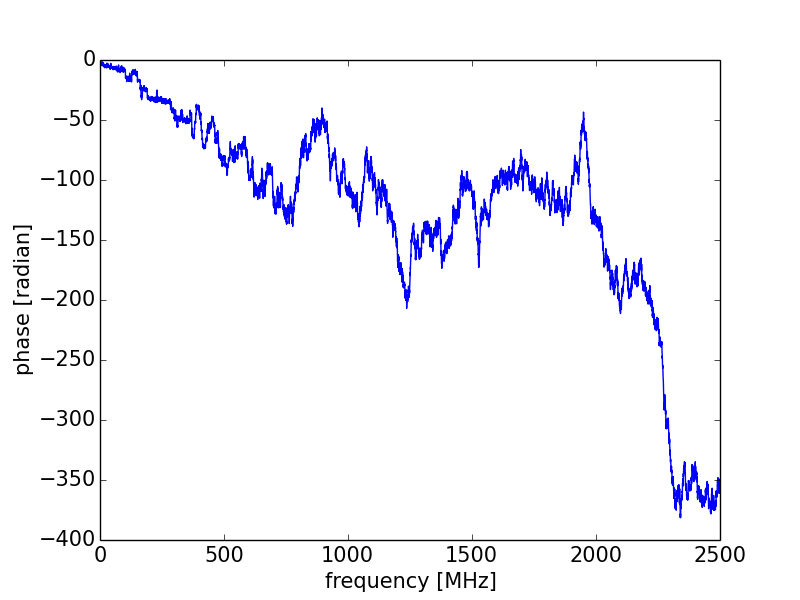
\includegraphics[width=0.32\linewidth]{nc_phase.png}}
  \caption{no capacitor case (left: spectrum, middle: ratio after/before, right: phase difference)}
  \label{fig:pdspec2}
\end{figure}
We  show an  example of  waveform for  the no  capacitor case  and the
distribution of  the difference  in the fig.~\ref{fig:m2ex}.  For this
method, the residuals are larger than for the first method.

\begin{figure}[!ht]
  \centering
  \hspace*{-3ex}
  \subfigure{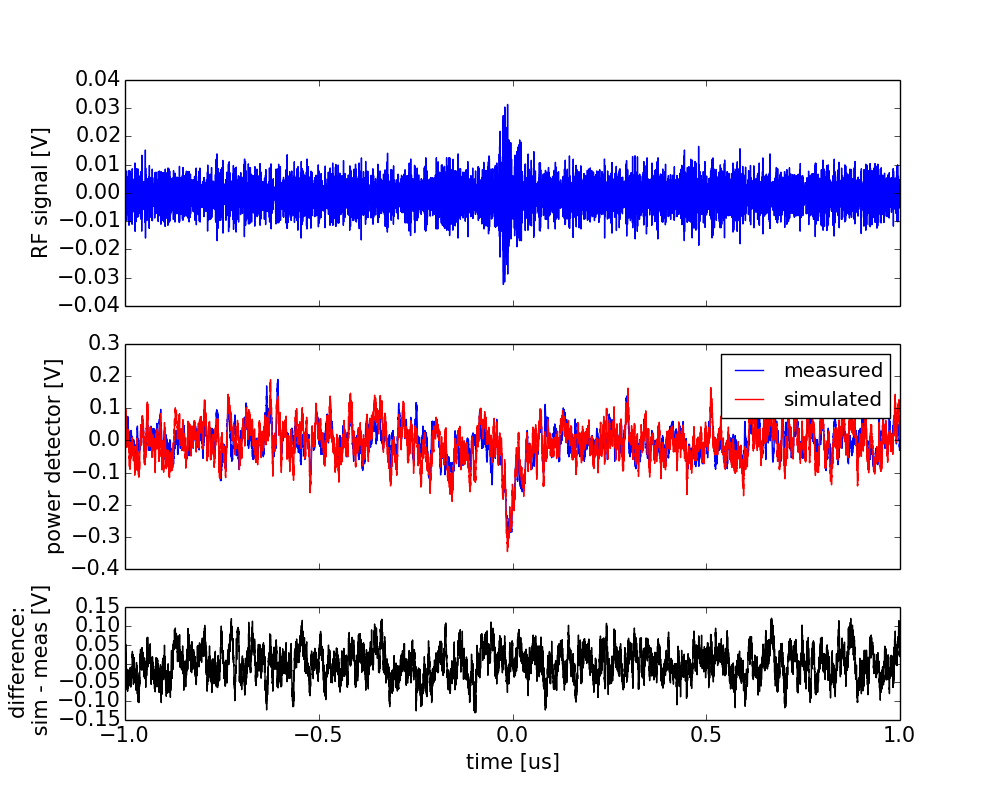
\includegraphics[width=0.49\linewidth]{nocapa_method2.png}}
  \subfigure{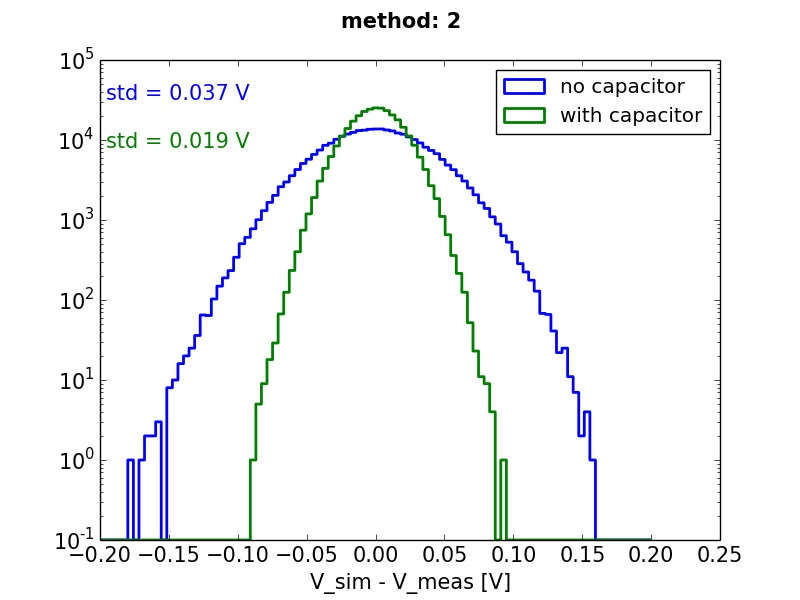
\includegraphics[width=0.49\linewidth]{res_method2.png}}
%  \subfigure{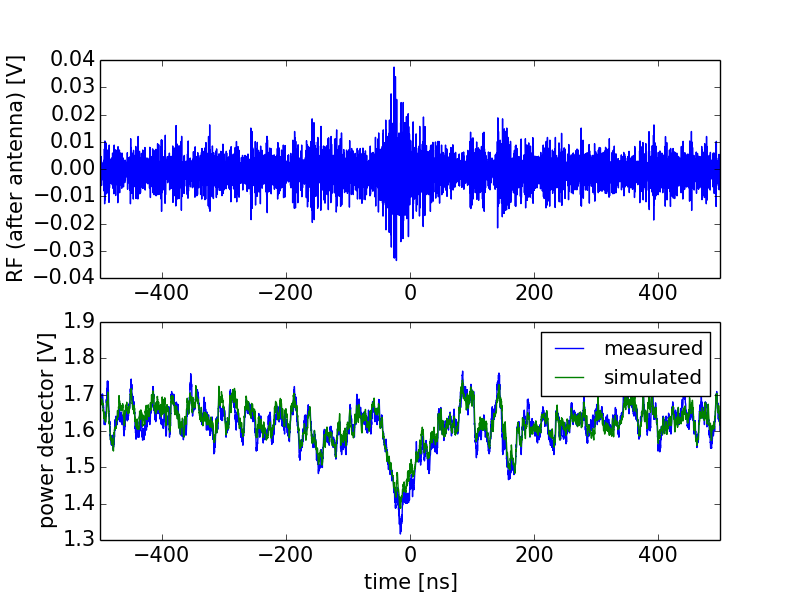
\includegraphics[width=0.49\linewidth]{examplepowerdetsim.png}}
%  \subfigure{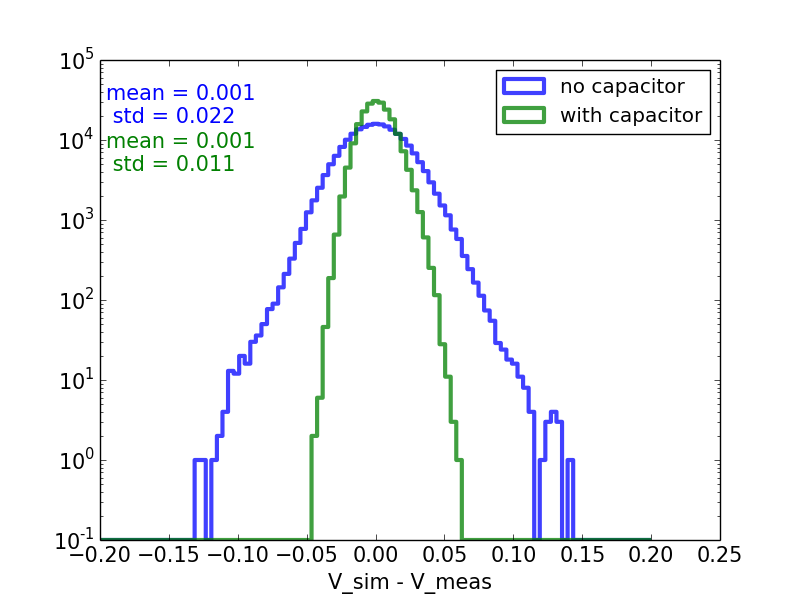
\includegraphics[width=0.49\linewidth]{residualpd.png}}
  \caption{}
  \label{fig:m2ex}
\end{figure}


\newpage
\paragraph{convolution with fixed parameters (method 3)}
For the first  method we had found that depending  on the waveform the
result for  the linear transformation parameters would  vary, which is
not really  meaningful.  We implemented  a third method which  is very
similar to the first one except  that we fix the DC caracterisitcs and
then we  fit the best $\tau$.   We use the relation  found between the
average the RF  waveform in dBm and the average  of the power detector
waveform (see  fig~\ref{fig:pdcarac}) and produce  the convolution the
same way as describe before.  The  decay time constant we find in this
case is  slightly different, we find  $\rm \tau_{capa} =  41.5 ns$ and
$\rm  \tau_{capa}   =  6.3  ns$.    The  results  are  shown   in  the
fig.~\ref{fig:m3ex}
\begin{figure}[!ht]
  \centering
  \hspace*{-3ex}
  \subfigure{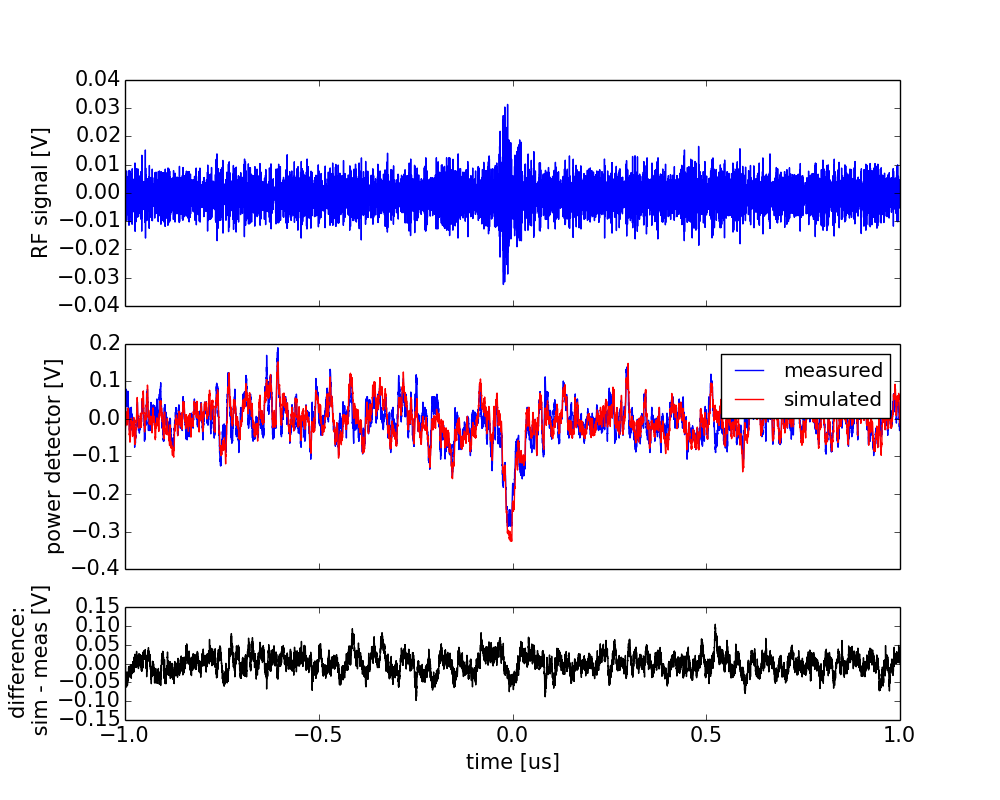
\includegraphics[width=0.49\linewidth]{nocapa_method3.png}}
  \subfigure{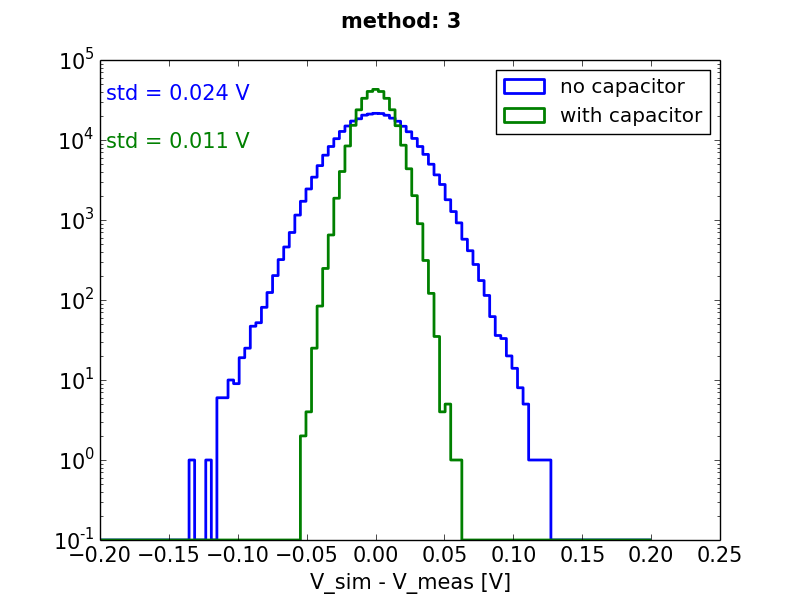
\includegraphics[width=0.49\linewidth]{res_method3.png}}
%  \subfigure{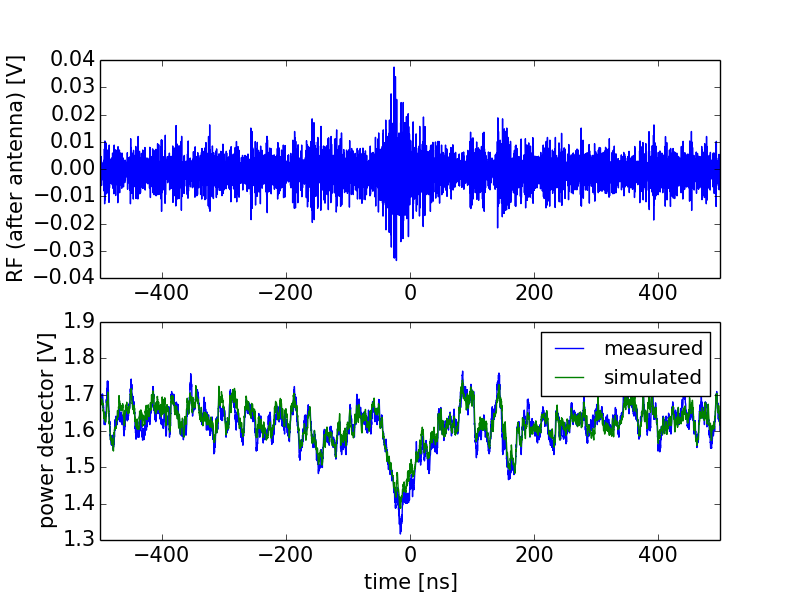
\includegraphics[width=0.49\linewidth]{examplepowerdetsim.png}}
%  \subfigure{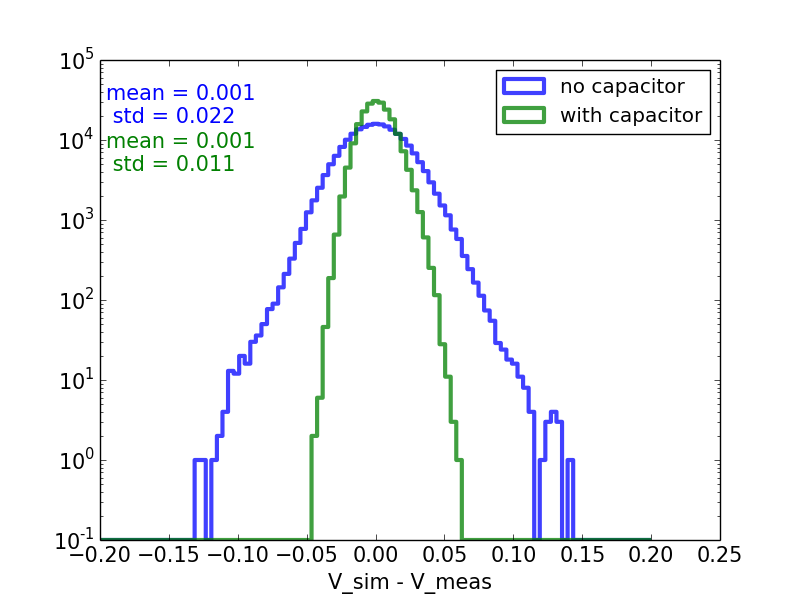
\includegraphics[width=0.49\linewidth]{residualpd.png}}
  \caption{}
  \label{fig:m3ex}
\end{figure}
The residuals  found with  this method  are as good  as for  the first
method.

\clearpage
\subsection{easier board}
This stage is  an amplification of the power  detector signal in order
to choose the dynamic range we want  to keep at the final stage. It is
performed with an amplifier and adjustable voltage offset.  Up to now,
this step  was simulated  with a linear  transformation.  We  will see
that  we  need to  account  for the  dependence  in  frequency of  the
amplifier.\\To determine the characteristics of this stage, we had set
up an experiment with a  C-band antenna followed by the power detector
and an EASIER board.  The signal was recorded after the power detector
and after the board  (see figure~\ref{fig:exampleboard}).  \\ First we
look  at the characteristics  $\rm <V_{board}>  = f(<V_{PD}>)$  of the
mean  value  of   the  waveforms  (see  figure~\ref{fig:carac}  left).
However,  when we  look at  the characteristics  for $\rm  V_{board} =
f(V_{PD})$  we obtain a  different result  (see figure~\ref{fig:carac}
right).   That  means  that  the  response for  the  DC  component  is
different  from  the  higher  frequencies, or  equivalently  that  the
amplifier gain is not flat in frequency.
\begin{figure}[!ht]
  \centering
  \hspace*{-3ex}
  \subfigure{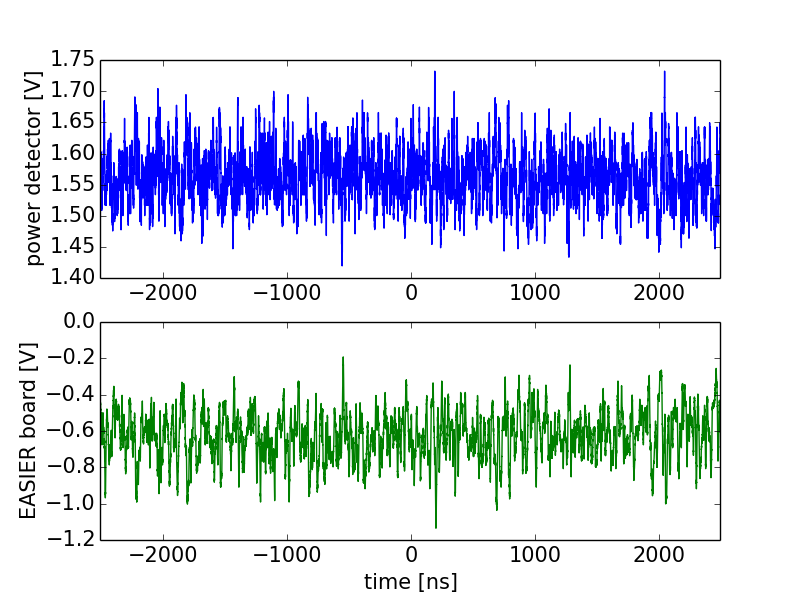
\includegraphics[width=0.60\linewidth]{exampleeasierboard.png}}
  \caption{example  of waveform  after  the power  detector (top)  and
    aftern the EASIER board (bottom) }
  \label{fig:exampleboard}
\end{figure}

\begin{figure}[!ht]
  \centering
  \hspace*{-3ex}
  \subfigure{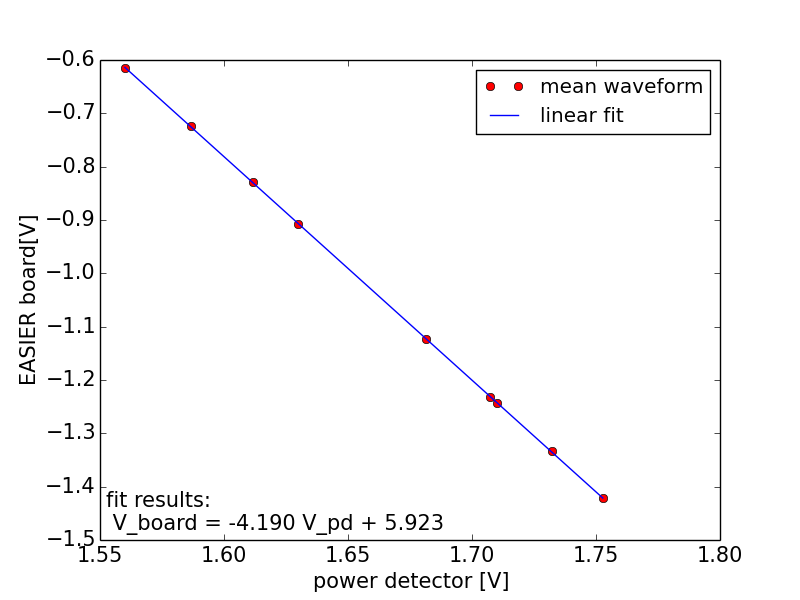
\includegraphics[width=0.45\linewidth]{boardcaracDC.png}}
  \subfigure{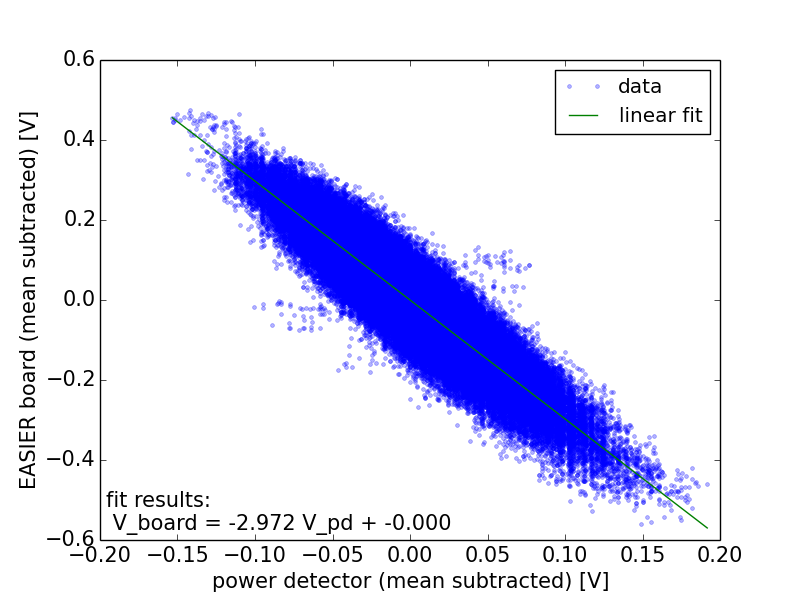
\includegraphics[width=0.45\linewidth]{boardcaracHF.png}}
  \caption{caracteristics of  the easier board for the  average of the
    waveform (left) or for all the points when the baseline is removed
    (right)}
  \label{fig:carac}
\end{figure}

We determine the  response in frequency of the  board taking the ratio
of the FFT of the waveforms.  An example of the FFT of one waveform is
shown in figure~\ref{fig:examplefft}.
\begin{figure}[!ht]
  \centering
  \hspace*{-3ex}
  \subfigure{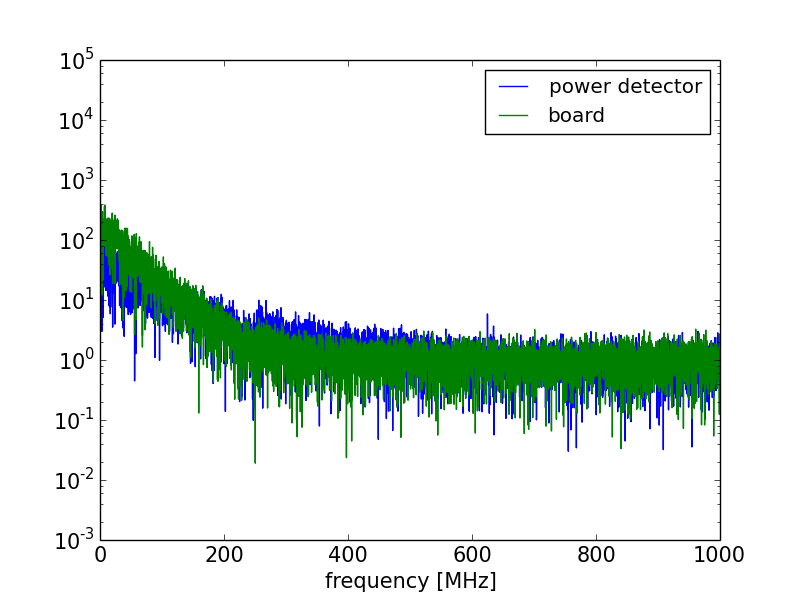
\includegraphics[width=0.32\linewidth]{fftexspec.png}}
  \subfigure{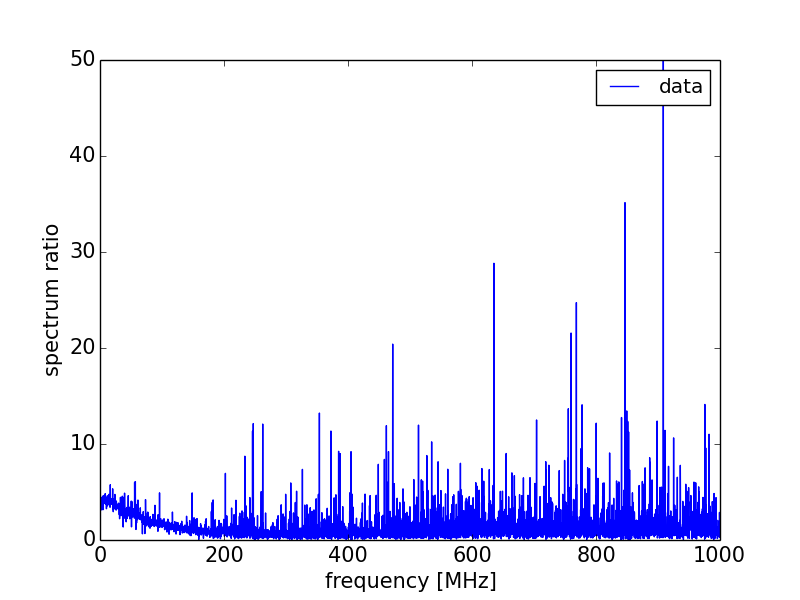
\includegraphics[width=0.32\linewidth]{fftexratio.png}}
  \subfigure{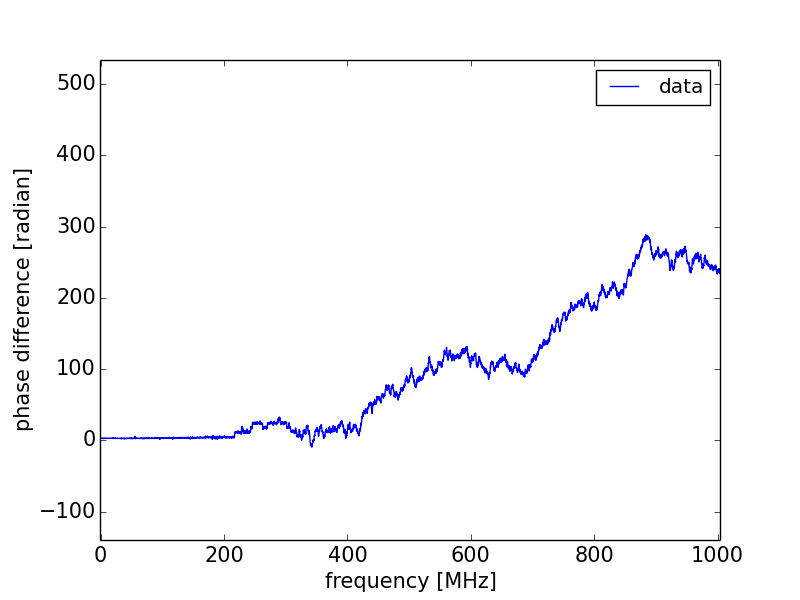
\includegraphics[width=0.32\linewidth]{fftexphase.png}}
  \caption{Left:  example of  spectra of  the power  detector  and the
    easier board. Middle: the ratio of the spectra on the left. Right:
    phase difference between the two fft.}
  \label{fig:examplefft}
\end{figure}
We see that  it is really noisy,  that's because it is FFT  of noise !
Most of  the power is in the  first 200MHz. For the  spectrum we could
average  over   multiple  spectra,   for  the  phase   we  encountered
difficulties to average  it due to phase jumps.  So  we fit an average
spectrum and fit only one phase.  Then to obtain the board signal from
the power detector the first step is to make the non DC frequencies go
through the response we found and then add the correct offset with the
$\rm <V_{board}>  = f(<V_{PD}>)$ characteristic.  \\  The fitted curve
shown in red on figure~\ref{fig:fitboard} are:
\begin{samepage}
  \begin{itemize}
  \item spectrum:  $\rm s = a\cdot  e^{-\frac{(x-\mu)^2}{2\sigma^2}} + k
    $\\ with a =  3.86, $\rm \mu = -40$ , $\rm \sigma =  75.1$ , k = 1.0
    and x is the frequency in MHz
  \item phase: $\rm p = ax^2 + bx + c $ \\ with a = 4.8 $\rm 10^{-5}$, b
    = -1.1 $\rm 10^{-3}$, c = 2.97
  \end{itemize}
\end{samepage}

\begin{figure}[!ht]
  \centering
  \hspace*{-3ex}
  \subfigure{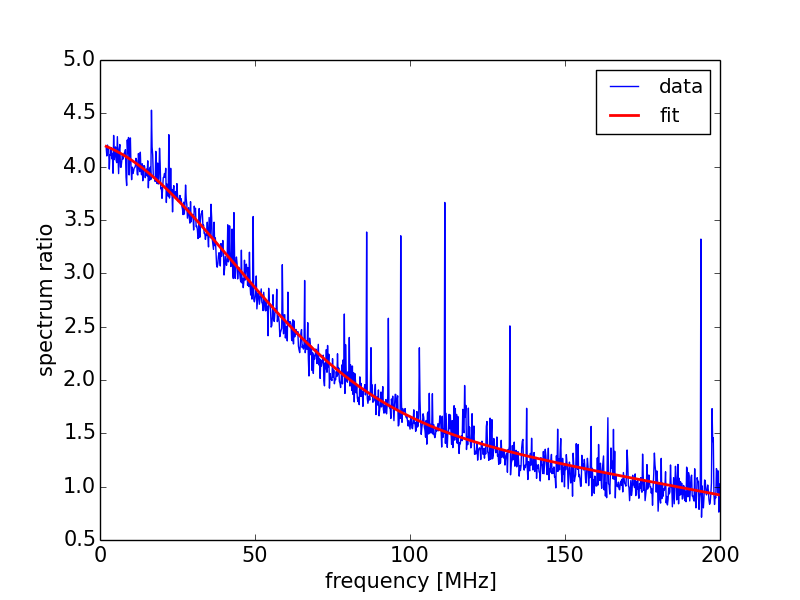
\includegraphics[width=0.45\linewidth]{fitspecboard.png}}
  \subfigure{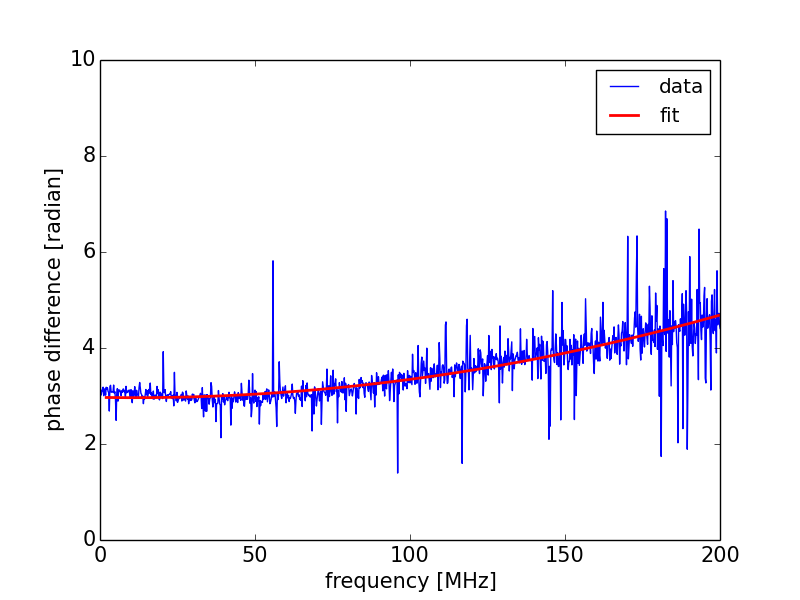
\includegraphics[width=0.45\linewidth]{fitphaseboard.png}}
  \caption{Fit of the board response (spectrum on the left, phase on the left), function and parameters are given in the text}
  \label{fig:fitboard}
\end{figure}

Now we  can look at the  comparison between the old  simulation with a
constant gain and  the new method with a  frequency dependent gain. An
example of waveforms (measured, simulated  with old and new method) is
shown in  figure~\ref{fig:simboard} left and  the difference histogram
is given on the right.
\begin{figure}[!ht]
  \centering
  \hspace*{-3ex}
  \subfigure{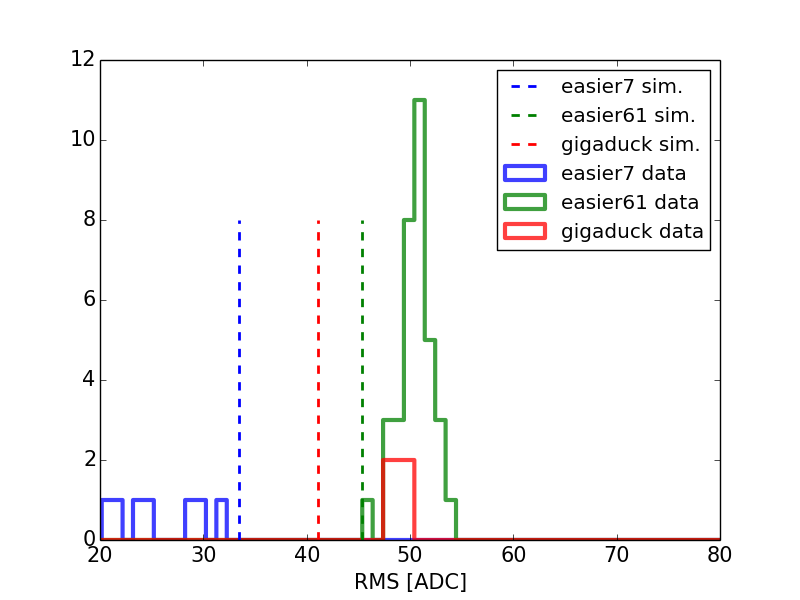
\includegraphics[width=0.33\linewidth]{datasimrmsdist.png}}
  \subfigure{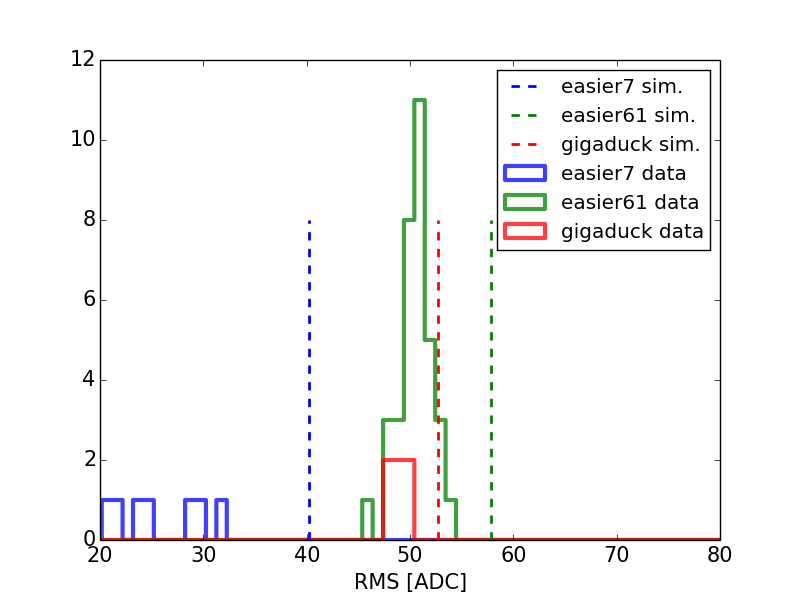
\includegraphics[width=0.33\linewidth]{m2_datasimrmsdist.png}}
  \subfigure{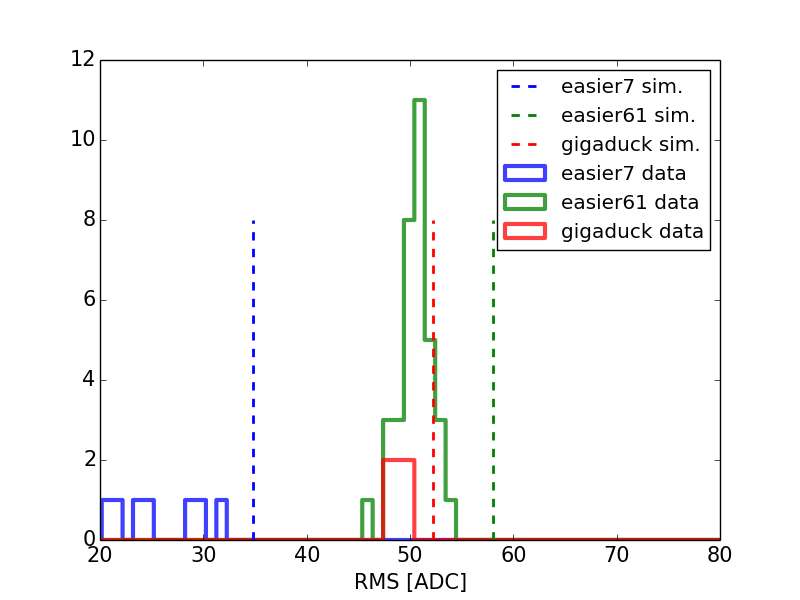
\includegraphics[width=0.33\linewidth]{m3_datasimrmsdist.png}}
  \caption{comparison of the measured distribution of amplitude and the simulated one.}
  \label{fig:datatrace}
\end{figure}


\begin{figure}[!ht]
  \centering
  \hspace*{-3ex}
  \subfigure{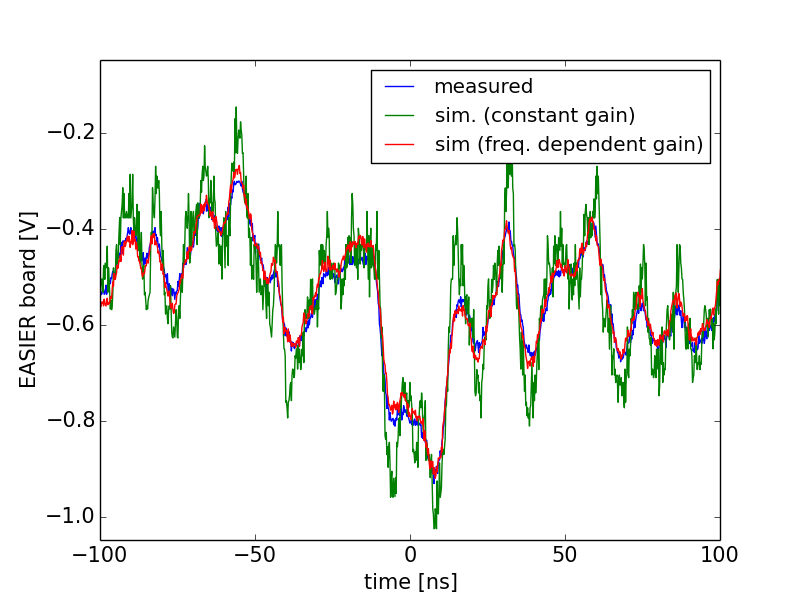
\includegraphics[width=0.45\linewidth]{examplesimboard.png}}
  \subfigure{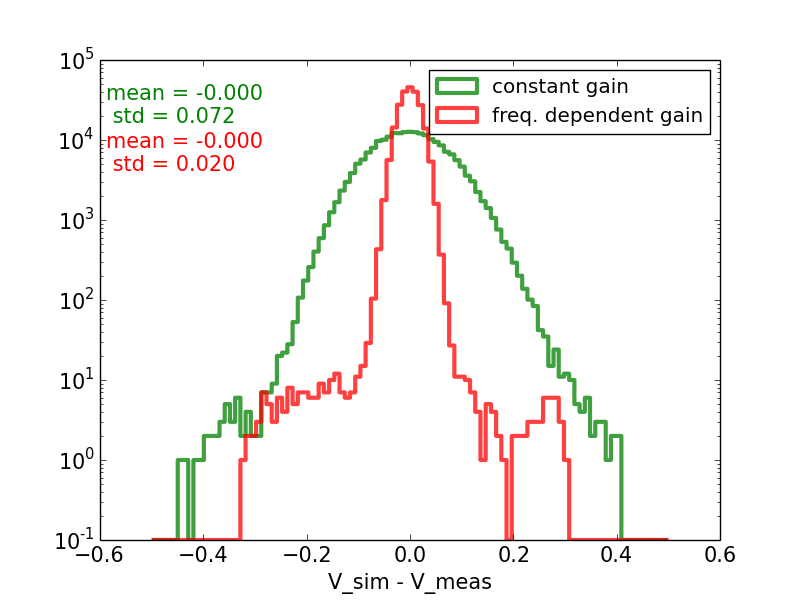
\includegraphics[width=0.45\linewidth]{residualboard.png}}
  \caption{left:waveforms  (measured  and  simulated), right:  voltage
    difference of around 20 waveforms}
  \label{fig:simboard}
\end{figure}

\newpage
\subsection{SD front end}
This is  the last piece  of the electronics  chain. We don't  have any
data to look  at its response.  From the Auger  technical report it is
composed of a  low pass filter ($\rm f_{cut}  = 20~MHz$).  We simulate
it with a butterworth filter of 4th order.



\section{Comparison data simulation}
Now that  we have a  good simulation of  each step of  the electronics
chain, we  want to test  the simulation with  the data. One way  to do
that is  by looking at  the fluctuations of  the radio signal  that we
measure in the recorded events. So we will carry out a full simulation
and compare the distribution of the  radio signal in ADC units. 
\subsection{data}
To measure the RMS of the  detectors installed in the field, we select
events with EASIER stations hit  and just histogram the radio waveform
in ADC (after  removing the baseline). We have  picked arbitrarely the
month  of  April 2015  (it  is  the period  when  all  the arrays  are
present).  We  show as an example  3 waveforms, one for  each array of
the C-band  in the  figure~\ref{fig:datatrace} (left) and  the average
RMS  is shown  for all  the stations  during the  chosen month  in the
figure~\ref{fig:datatrace} (right). Most of the EASIER61 detector have
their RMS around  50 ADCs and some  of them are a little  off and some
close to  zero.  For the  EASIER7 array the  RMS is lower  because the
capacitor  is  present after  the  power  detector.   Finally all  the
GIGADUCK detectors (except one) have their RMS between 47 and 50 ADCs.

\begin{figure}[!ht]
  \centering
  \hspace*{-3ex}
  \subfigure{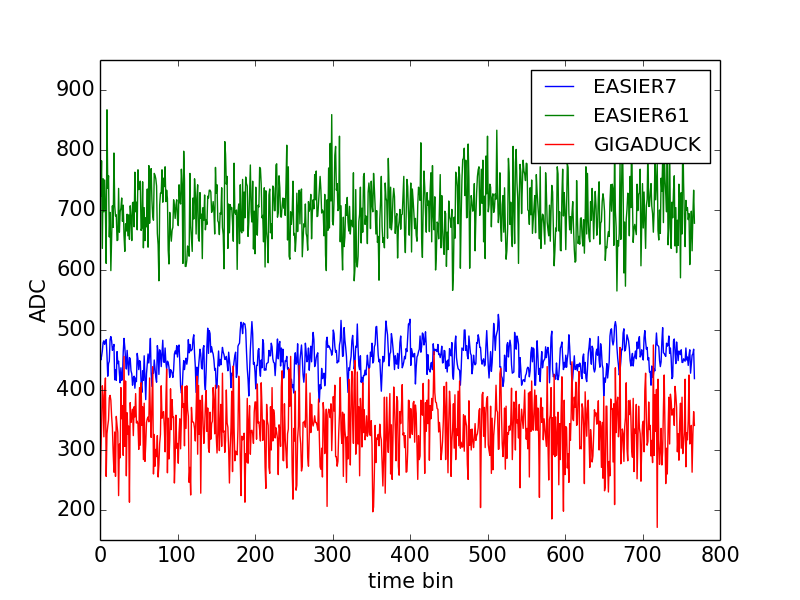
\includegraphics[width=0.49\linewidth]{datatrace.png}}
  \subfigure{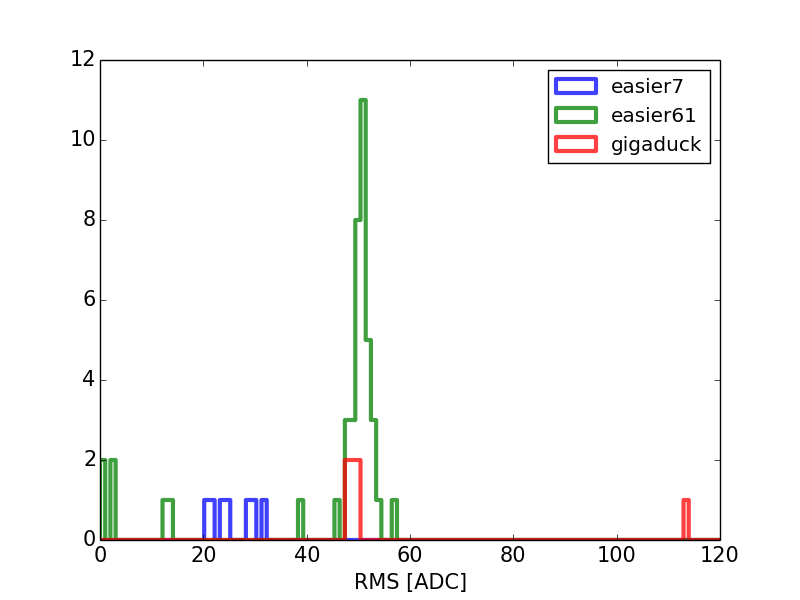
\includegraphics[width=0.49\linewidth]{datarmsdist.png}}
  \caption{example of trace from each detector in the C-band. right: distribution of the average RMS of all detectors}
  \label{fig:datatrace}
\end{figure}

\begin{figure}[!ht]
  \centering
  \hspace*{-3ex}
  \subfigure{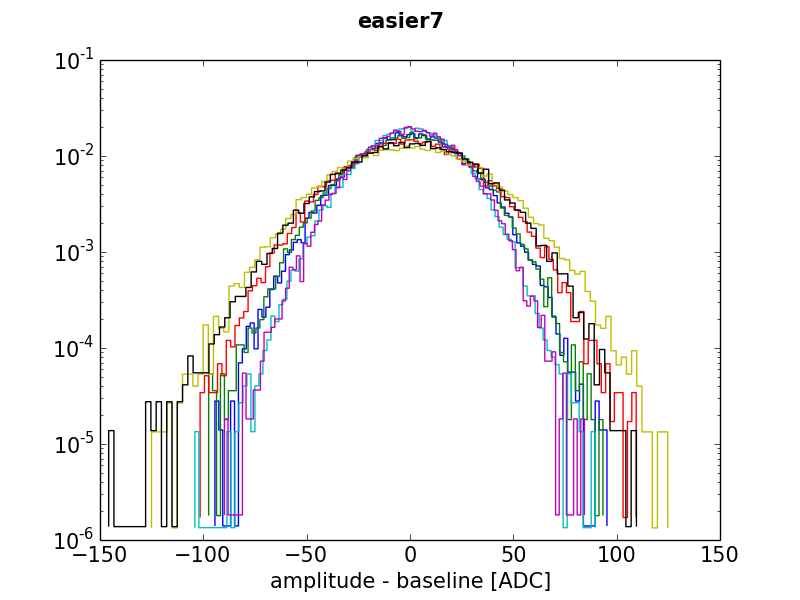
\includegraphics[width=0.32\linewidth]{disteasier7.png}}
  \subfigure{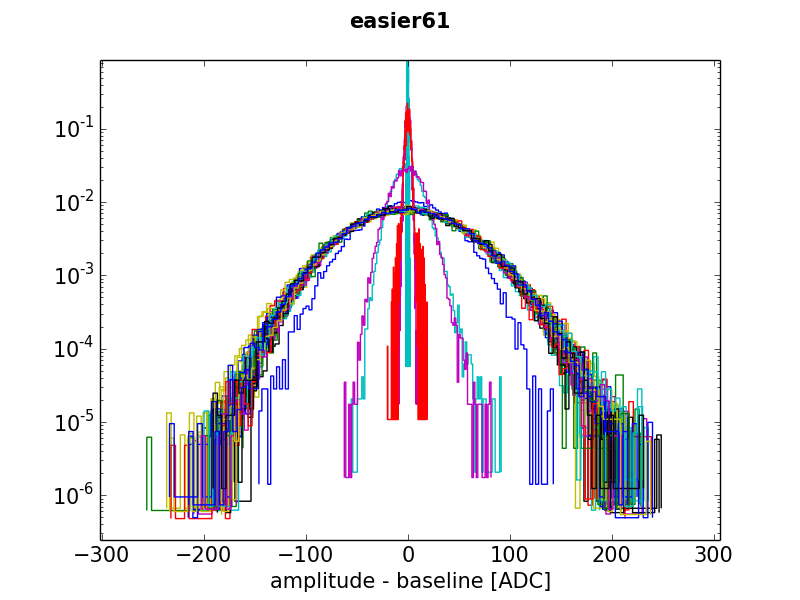
\includegraphics[width=0.32\linewidth]{disteasier47.png}}
  \subfigure{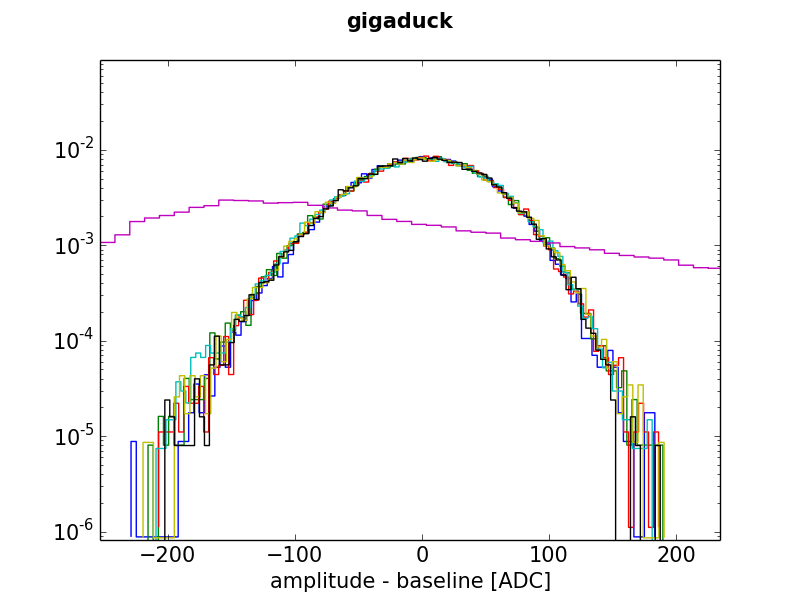
\includegraphics[width=0.32\linewidth]{distgigaduck.png}}
  \caption{example of  trace from each detector in  the C-band. right:
    distribution of the average RMS of all detectors.}
  \label{fig:datatrace}
\end{figure}

\subsubsection{simulation}
Now    we   can    produce    HF   waveforms    from   the    measured
spectra~\ref{sec:rf},   then  make   the  waveform   go   through  the
electronics  simulation we  described  in section~\ref{sec:elec}.   We
show  here  the  results  for  the three  methods  of  power  detector
simulation.    Figure~\ref{fig:m1_distdata},   ~\ref{fig:m2_distdata},
~\ref{fig:m3_distdata} show the measured and simulated distribution of
amplitude in ADC counts, and figure~\ref{fig:compmeanrms} compares the
average RMS (we removed the bad stations).

\begin{figure}[!ht]
  \centering
  \hspace*{-3ex}
  \subfigure{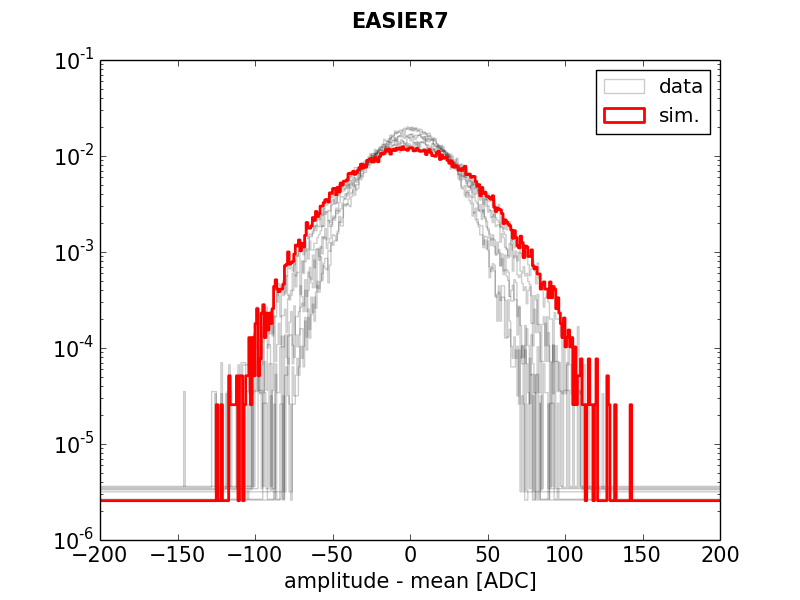
\includegraphics[width=0.32\linewidth]{m1_distdatasimEA7.png}}
  \subfigure{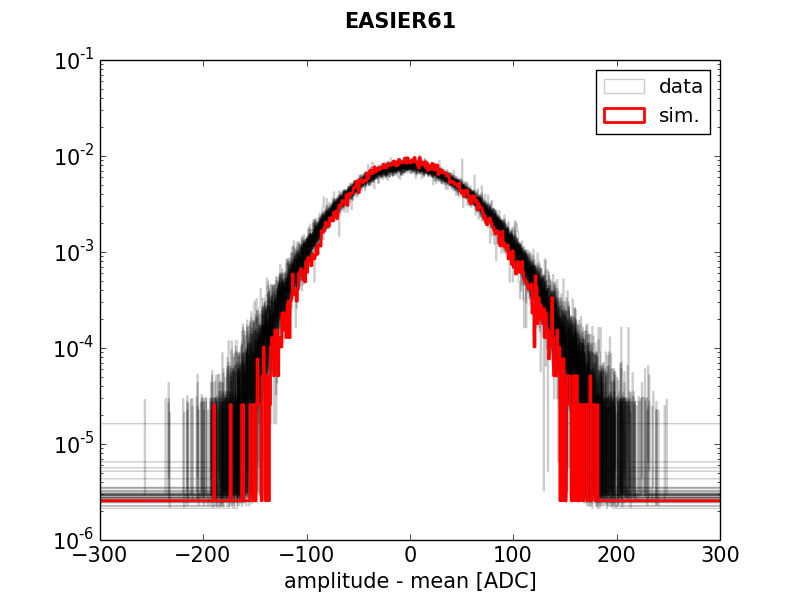
\includegraphics[width=0.32\linewidth]{m1_distdatasimEA61.png}}
  \subfigure{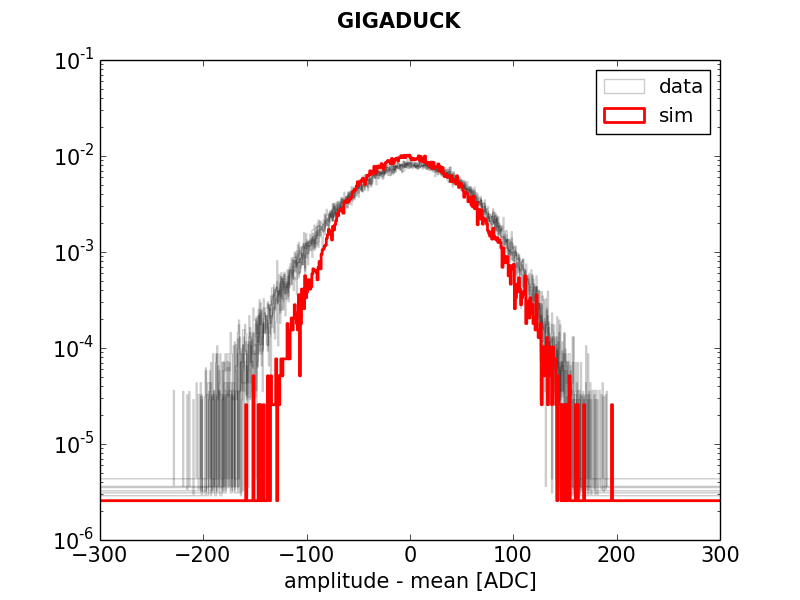
\includegraphics[width=0.32\linewidth]{m1_distdatasimGD.png}}
  \caption{method 1: comparison of the measured distribution of amplitude and the simulated one.}
  \label{fig:m1_distdata}
\end{figure}

\begin{figure}[!ht]
  \centering
  \hspace*{-3ex}
  \subfigure{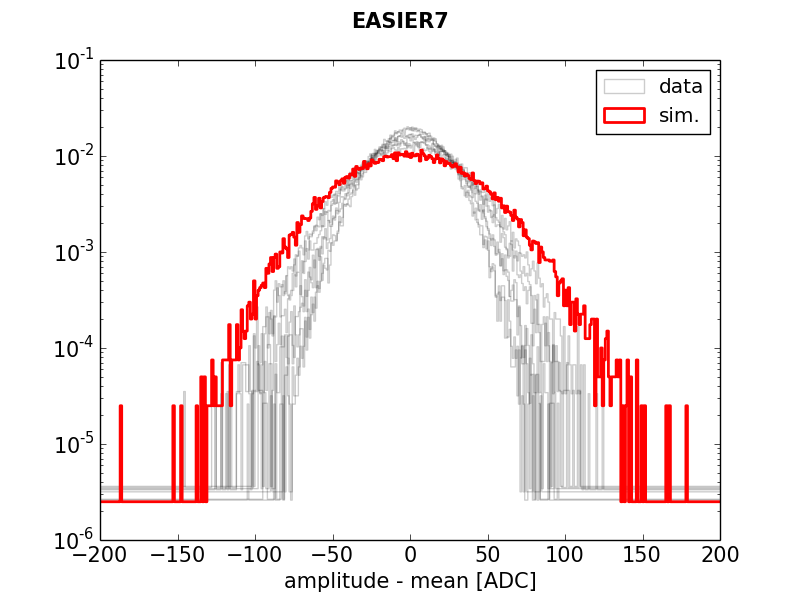
\includegraphics[width=0.32\linewidth]{m2_distdatasimEA7.png}}
  \subfigure{\includegraphics[width=0.32\linewidth]{m2_distdatasimEA61.png}}
  \subfigure{\includegraphics[width=0.32\linewidth]{m2_distdatasimGD.png}}
  \caption{method 2: comparison of the measured distribution of amplitude and the simulated one.}
  \label{fig:m2_distdata}
\end{figure}

\begin{figure}[!ht]
  \centering
  \hspace*{-3ex}
  \subfigure{\includegraphics[width=0.32\linewidth]{m3_distdatasimEA7.png}}
  \subfigure{\includegraphics[width=0.32\linewidth]{m3_distdatasimEA61.png}}
  \subfigure{\includegraphics[width=0.32\linewidth]{m3_distdatasimGD.png}}
  \caption{method 3: comparison of the measured distribution of amplitude and the simulated one.}
  \label{fig:m3_distdata}
\end{figure}

\begin{figure}[!ht]
  \centering
  \hspace*{-3ex}
  \subfigure{\includegraphics[width=0.33\linewidth]{datasimrmsdist.png}}
  \subfigure{\includegraphics[width=0.33\linewidth]{m2_datasimrmsdist.png}}
  \subfigure{\includegraphics[width=0.33\linewidth]{m3_datasimrmsdist.png}}
  \caption{comparison of the measured distribution of amplitude and the simulated one.}
  \label{fig:datatrace}
\end{figure}

At the  end, the three method  give very close results,  the first one
yields a larger RMS for the  capacitor case, but a smaller one for the
non capacitor case.  The two  other give consistantly a larger RMS for
the three  detector configurations. Note that the  difference is quite
small, only  a few ADC  counts.  (50  ADC is 1dB  and we have  at most
differences of around 15 ADC i.e. less than 10$\rm \%$)
%% At the  end, none of  the method finds  the correct value. But  we get
%% numbers very close to the data. 



%% At the end  the average value of the RMS are  smaller for EASIER61 and
%% GIGADUCK and larger for EASIER7. I  think that the reason might be the
%% parameters found in  section 1. When I fit the  time constant I obtain
%% at  the  same time  the  characteristic of  the  power  detector (V  =
%% f(power)). When we look  at the value a and b obtain  for the two case
%% we see that they are different and the final fluctuation are sensitive
%% to  the parameter  a  (the slope).   Especially  we see  that for  the
%% capacitor case the  slope is larger than the  no capacitor case, which
%% goes in the  same trend as the  discrepancy in the RMS (I  mean if the
%% value of a was taken as the  mean of the two value we would reduce the
%% discrepancies of both cases.) Another possibility is that the response
%% is a  little different for the noise  part and the signal  part. In my
%% thesis I had found a difference  in the fit results for the noise part
%% and the signal part. 
 



\section*{conclusion}
We  have  gone  through  the  different step  to  simulate  an  EASIER
waveform.  In  particular, we  have detailed the  generation of  an RF
waveform from a realistic spectrum. We also improved the simulation of
the  adaptation  electronics. The  full  simulation  is then  compared
against  data looking at  the traces  fluctuation in  ADC.  We  find a
simulated waveform overestimated the  fluctuation by a small number of
ADC.

%%\section{Understanding the fluctuations}
We have  looked at the waveform  fluctutations because it is  a way to
check the  detector's simulation. But it  is also important  to get an
idea of  the detector  sensitivity. There is  the formula given  for a
square law detector:
\begin{equation}
  F = \frac{k_{B} T_{sys}}{\sqrt{\Delta B \tau}}
  \label{eq:sensitivity}
\end{equation}
This formula  is in fact the  ratio of the  RMS of a square  law radio
detector and an integration term (similar to a $\sqrt{N}$).  It states
that the  minimum observable signal  (or the detector  sensitivity) is
the   system  noise   temperature  reduced   by  how   much   you  can
integrate/average it. In  reality it is a good figure  of merit but it
is    not   completely    correct    for   all    the   cases.     The
equation~\ref{eq:sensitivity} is only  correct when the integration is
done  by a numerical  filter with  the frequency  $\frac{1}{\tau}$. We
want to understand better this formula, several cases are discussed in
the following paragraphs.


\subsection{case study}
\paragraph{derivation of the equation}
The  derivation of  the formula~\ref{eq:sensitivity}  is given  in the
book    "Tools   of    Radio   Astronomy"    (T.L~Wilson,   K.~Rohlfs,
S.~Huttemeister).  One wants  to find  the what  is the  value  of the
detectable  signal,  so we  look  at  the  standard deviation  of  the
recorded signal. The main steps are the following:
\begin{itemize}
\item take a radio detector with a bandwidth B, the amplitude of the signal $v(t)$ follows a gaussian distribution.
\item the signal goes through a square law detector $y = av(t)^2$. One
  can  compute the  mean  and  standard deviation  and  finds: $<y>  =
  a\sigma_v^2$ and $\sigma_y = \sqrt{2}a\sigma_v^2$ (with $<v^2> = <power> =
  kT_{sys}     G    B$).    (this     webpage    might     also    help:
  http://mathworld.wolfram.com/GaussianIntegral.html)
\item So we have: $\sigma_y = \sqrt{2} <y> $ , with $\sigma_y = k_B \Delta
  T G B$ so $\Delta T = \sqrt{2} T_{sys}$
\item now  if we  average over  a time $\tau$,  that means  we average
  over$ N = f_{Nyquist}*\tau$ points where $f_{Nyquist} = 2B$, and we reduce the fluctuation by a factor $\sqrt{N}$
\item we finally obtain: $\Delta T = \frac{T_{sys}}{\sqrt{B\tau}}$
\end{itemize}

So to  sum up, for  a input gaussian  signal followed by a  square law
detector we expect the  ratio $\rm \frac{\sigma}{\mu} = \sqrt{2}$. And
this  ratio  is then  modified  by  the  later processing,  averaging,
filtering.

\paragraph{ideal case}
Let's take the simple  case of a square law detector with
a bandwidth of  [0 - 2GHz] for instance.  We  produce a noise waveform
with a flat spectrum and look  at the distribution of the power in the
figure~\ref{fig:noise}.
\begin{figure}[!ht]
  \centering
  \hspace*{-3ex}
  \subfigure{\includegraphics[width=0.60\linewidth]{noise.png}}
  \caption{}
  \label{fig:noise}
\end{figure}
We  can check that  the ratio  $\rm \frac{\sigma}{\mu}  $ is  equal to
$\sqrt{2}$.   Now if we  average with  a numerical  filter with  a cut
frequency  $f_{cut} =  1/\tau$ we  see  that it  follows the  expected
equation on the figure~\ref{fig:ratiofilter}. 
\begin{figure}[!ht]
  \centering
  \hspace*{-3ex}
  \subfigure{\includegraphics[width=0.60\linewidth]{rationumfilter.png}}
  \caption{}
  \label{fig:ratiofilter}
\end{figure}

\paragraph{bandwidth effect}
Now  we can  also look  at the  changes on  the fluctuations  when the
bandwidth  is  reduced.   Figure~\ref{fig:bw}  (left) shows  the  $\rm
\frac{\sigma}{\mu} $ ratio when we  keep the maximum frequency to 2GHz
but we reduce the lower bound  to reduce the bandwidth. The ratio stay
$\sqrt{2}$.   But  when we  filter,  we  see  discrepancy between  the
expected  ratio   and  the  simulated   one  (see  figure~\ref{fig:bw}
(right)). We see  that if we reduce the bandwidth,  the ratio is lower
than  expected and  plateaus at  for the  high frequency  filters (low
$\tau$) but  matches the  formulas at the  low frequency  filter (high
$\tau$).  This can be understood when we think about the FFTs (or look
at them  on figure~\ref{fig:fft}). The fourier transform  of the power
for  a signal  at frequencies  between [f1  - f2]  has  a contribution
between [0 ;  $\Delta B/2$] and another one between  [2*f1 ; 2*f2]. On
the  figure we  see  an example  for an  input  spectrum of  [1.5 ;  2
  GHz]. If we  filter with a frequency $f_{cut}  $smaller than $\Delta
B/2$ we follow the equation because we have a full bandwidth from [0 ;
  $f_{cut}$], if $f_{cut}$  is larger then we go into  the hole in the
power spectrum and  we don't add any frequency  in the average, that's
why the ratio goes to a constant.

\begin{figure}[!ht]
  \centering
  \hspace*{-3ex}
  \subfigure{\includegraphics[width=0.45\linewidth]{ratiodiffBW.png}}
  \subfigure{\includegraphics[width=0.45\linewidth]{rationumfilterdiffBW.png}}
  \caption{left: ratio $\frac{\sigma}{\mu}$ versus the lower frequency
    $f_min$ of the noise spectrum. rigt: the ratio when we apply a low
    pass filter of frequency cut $f_{cut}= 1/\tau$ to the power. It is
    shown for three different $f_{min}$}
  \label{fig:bw}
\end{figure}

\begin{figure}[!ht]
  \centering
  \hspace*{-3ex}
  \subfigure{\includegraphics[width=0.60\linewidth]{specnoise.png}}
  \caption{example of spectra of the  amplitude and power for an input
    noise signal. We see the two contribution in the spectrum of the power, and the hole if $\Delta B/2 \leq f_{min}$}
  \label{fig:fft}
\end{figure}


\paragraph{sliding window}
If instead of  filtering by cutting the frequency  spectrum we average
over  several bins,  i.e. a  sliding window  average.  If  we consider
$\tau$ as  the window size we  see (fig~\ref{fig:slidingwindow}) that
the ratio  doesn't follow the equation~\ref{sensitivity}.  There is an
additional factor  to be  added.  This shows  that the  formula really
depends on the processing, and one  should use it as a figure of merit
or a rough estimation.
\begin{figure}[!ht]
  \centering
  \hspace*{-3ex}
  \subfigure{\includegraphics[width=0.60\linewidth]{slidingwindow.png}}
  \caption{$\frac{\sigma}{\mu}$ ratio after  applying a sliding window
    of size $\tau$ for different $f_{min}$}
  \label{fig:slidingwidow}
\end{figure}

%%\section*{conclusion}
We  have  gone  through  the  different step  to  simulate  an  EASIER
waveform.  In  particular, we  have detailed the  generation of  an RF
waveform from a realistic spectrum. We also improved the simulation of
the  adaptation  electronics. The  full  simulation  is then  compared
against  data looking at  the traces  fluctuation in  ADC.  We  find a
simulated waveform overestimated the  fluctuation by a small number of
ADC.

%\include{signal/signal}
%\include{limit/limit}
\addcontentsline{toc}{chapter}{Bibliography}                                 
\bibliographystyle{atlasnote}
\bibliography{easier}
%% \newpage
%% \begin{thebibliography}{9}
%% \bibitem{gorham}P. W. Gorham et al., Phys. Rev. D 78, 032007 (2008).
%%   [arXiv:0705.2589 [astro-ph]]
%% \bibitem{augerpolar} The Pierre Auger Collaboration, Phys. Rev. D 89, 052002 (2014)
%% \bibitem{crome}
%% \end{thebibliography}

\end{document}
